\documentclass[a4paper,11pt]{article}
\usepackage{setspace}
\usepackage[utf8]{inputenc}
%\usepackage{subfigure}

\pagestyle{plain}

\usepackage{amssymb, bm, blkarray, multicol}
\usepackage{listings,xcolor,lmodern}
\usepackage{graphicx}
\usepackage{enumitem}
\usepackage{tikz}
\usepackage{booktabs}
\usepackage{amsmath}
\usepackage{algorithm}
\usepackage{algpseudocode}
\usepackage[nottoc]{tocbibind}
\usepackage{upgreek}

\usepackage{mathtools}
\mathtoolsset{showonlyrefs}

\usepackage{hyperref}
\usepackage{url}
\usepackage{nicefrac}
\usepackage{microtype}

\usepackage{latexsym}
% \usepackage{a4wide}

\newtheorem{theorem}{THEOREM}
\newtheorem{lemma}[theorem]{LEMMA}
\newtheorem{corollary}[theorem]{COROLLARY}
\newtheorem{proposition}[theorem]{PROPOSITION}
\newtheorem{remark}[theorem]{REMARK}
\newtheorem{definition}[theorem]{DEFINITION}
\newtheorem{fact}[theorem]{FACT}

\newtheorem{problem}[theorem]{PROBLEM}
\newtheorem{exercise}[theorem]{EXERCISE}
\def \set#1{\{#1\} }

\lstset{
  basicstyle=\ttfamily,
  columns=fullflexible,
  frame=single,
  breaklines=true,
  postbreak=\mbox{\textcolor{red}{$\hookrightarrow$}\space},
}

\newcommand{\E}{\mathbb{E}}
\newcommand{\var}{\mathrm{Var}}
\newcommand{\cov}{\mathrm{Cov}}
\newcommand{\KL}{\mathrm{KL}}
\newcommand{\neighb}{\text{ne}}
\DeclareMathOperator*{\argmax}{arg\,max}
\DeclareMathOperator*{\argmin}{arg\,min}
\newcommand{\Perp}{\mathrel{\text{\scalebox{1.07}{$\perp\mkern-10mu\perp$}}}}

\usetikzlibrary{shapes.geometric}

\title{  	{ 
\includegraphics[scale=.5]{figures/ucl_logo.png}}\\
{{\Huge Kernel Tests for Markov Chain Monte Carlo Methods}}\\
% {\large Subtitle}\\
		}
\date{September 2020}
\author{Andrew Wei Jiang\thanks{
{\bf Disclaimer:}
This report is submitted as part requirement for the MSc in Computational Statistics and Machine Learning at UCL. It is
substantially the result of my own work except where explicitly indicated in the text. The report may be freely copied and distributed provided the source is explicitly acknowledged.
\newline}
\thanks{
{\bf Acknowledgements:}
I am greatly indebted to my supervisors, Arthur Gretton, Peter Orbanz, and Heishiro Kanagawa, for their patience and wisdom in challenging times.
\newline}
\\ \\
\\ \\
Supervisors: Arthur Gretton, Peter Orbanz, Heishiro Kanagawa}

\begin{document}
\maketitle
\thispagestyle{empty}
\onehalfspacing

\newpage
\begin{abstract}
    In Bayesian statistics, Markov chain Monte Carlo (MCMC) algorithms provide flexible ways to sample from analytically intractable posterior distributions. However, inference based on MCMC methods suffers from two sources of error: lack of convergence and mistakes in implementation. While there are a variety of methods to detect the former, less attention has been devoted to the latter. We propose two two-sample tests for diagnosing MCMC implementation errors based on Maximum Mean Discrepancy (MMD). The MMD tests exhibit lower Type I/II error rates than the commonly used Geweke test \cite{geweke_getting_2004} and perform competitively with recently proposed alternatives in several experiments. On the other hand, the computational costs of both MMD tests are quadratic in the number of observations compared to linear or log-linear for existing tests. Finally, we provide some evidence that, unlike existing alternatives, the MMD tests generalize well to domains other than $\mathbb{R}^{d}$. Source code is available at \url{https://github.com/awjiang/mcmc-kernel-tests}.
\end{abstract}
\setcounter{page}{1}
\newpage

\tableofcontents
\newpage

\section*{Note on Notation}
Unless otherwise noted, probability distributions and random variables are always denoted by uppercase unbolded letters (X). In $\mathbb{R}^{d}$, unbolded lowercase symbols (x) denote scalars, bolded lowercase symbols ($\mathbf{x}$) denote vectors, and bolded uppercase symbols ($\mathbf{X}$) denote matrices. In other domains, unbolded symbols (x) are used generically to refer to constituent elements.

\newpage

\section{Introduction}
In Bayesian statistics, given the prior distribution of the parameters $P(\mathbf{\Theta})$ and the likelihood of the observed data $P(\mathbf{Y} | \mathbf{\Theta})$, we are interested in sampling from the posterior distribution
\begin{equation}
    P(\theta | y) = \frac{P(y | \theta)P(\theta)}{P(y)} \propto P(y | \theta)P(\theta)
    \label{eq:posterior}
\end{equation}
for inference. When the normalizer $P(y)$ is analytically intractable, directly sampling from $P(\theta | y)$ is impossible. Instead, Markov chain Monte Carlo (MCMC) algorithms draw dependent samples from a Markov chain with $P(\theta | y)$ as its stationary distribution, only requiring the density to be known up to a constant of proportionality. On the other hand, their stochastic nature makes MCMC algorithms potentially difficult to work with. For instance, valid inference requires the eponymous Markov chain to converge to its stationary distribution, but the user may stop the algorithm before it has `burned in'. To avoid this pitfall, a variety of convergence diagnostics have been proposed in the literature. However, fewer studies have addressed the more fundamental issue of determining whether the implementation itself is correct; even if the algorithm has converged, it may not have the correct stationary distribution. Subtle errors can escape inspection by eye, particularly when the underlying algorithm is complex; worse still, they may subsequently propagate through the literature. For example \cite{del_negro_time_2015} and \cite{karlsson_corrigendum_2017} correct two highly cited MCMC algorithms in the econometrics literature --- over a decade after their initial publications. Thus, the development of principled tests to verify MCMC correctness is of significant importance to researchers.

There are a handful of MCMC correctness tests in the literature; in fact, the errors in \cite{del_negro_time_2015} and \cite{karlsson_corrigendum_2017} were initially detected using the Geweke test \cite{geweke_getting_2004}. However, these tests rely on testing a finite family of hypotheses based on scalar quantities derived from samples. If none of the hypotheses are rejected, then the test concludes that the sampler is error-free. In many cases, testing the correctness of, for instance, all first and second moments of the parameters, may be sufficient for the user. However, these tests will fail to detect any error not captured by the specified hypotheses. In this study, we introduce two tests based on Maximum Mean Discrepancy (MMD) in Reproducing Kernel Hilbert Spaces (RKHS) that can in theory detect any error in an MCMC algorithm, given the right kernel. The tests perform competitively with existing alternatives in a variety of settings, though they are more expensive to conduct, with a computational cost quadratic in the number of samples compared to linear or log-linear for existing tests. We show that kernel choice and the inclusion of hand-picked features relevant to MCMC can dramatically improve test power. In addition, unlike other tests, the MMD tests can be applied natively in domains other than $\mathbb{R}^{d}$.

\label{section:intro}
\section{Background}
\subsection{Markov Chain Monte Carlo (MCMC)}
MCMC algorithms sample from a target distribution $P$ by drawing dependent samples from a Markov chain with the same stationary distribution. They do not require the normalizer of the distribution to be known. Under certain conditions \cite{jones_markov_2004}, a Markov chain central limit theorem holds. Given a realization of a Markov chain $\{x_{1}, x_{2}, \ldots, x_{N}\}$ with stationary distribution $P$ and some real-valued function $g:\mathcal{X} \rightarrow \mathbb{R}$ with finite variance, let $\mu = \E_{P}[g(X)]$ and $\hat{\mu}^{(N)} = \frac{1}{N} \sum_{i=1}^{N}g(x_{i})$. Then
\begin{equation}
    \sqrt{N}(\hat{\mu}^{(N)} - \mu) \overset{D}{\rightarrow} \mathcal{N}(0, \sigma^{2})
    \label{eq:mcmc_clt}
\end{equation}

Other than in their target distributions, MCMC algorithms primarily differ in how they construct their Markov chains. We illustrate several methods below in $\mathbb{R}^{d}$.

\subsubsection{The Metropolis-Hastings Algorithm}
The Metropolis-Hastings algorithm \cite{metropolis_equation_1953,hastings_monte_1970} constructs a Markov chain with a desired stationary distribution $P$. Let $T(\mathbf{X} \rightarrow \mathbf{X}')$ denote the transition probability from state $\mathbf{X}$ to $\mathbf{X'}$ for an ergodic Markov chain. If $P$ satisfies the detailed balance condition
\begin{equation}
   T(\mathbf{X} \rightarrow \mathbf{X}') P(\mathbf{X}) = T(\mathbf{X}' \rightarrow \mathbf{X}) P(\mathbf{X}')
   \label{eq:dbc}
\end{equation}
then the Markov chain is reversible and has unique stationary distribution $P$. 

At every iteration, the algorithm draws a proposal $\mathbf{X}'$ from a proposal distribution $q$, which is required to have non-zero measure on the support of $P$. $\mathbf{X}'$ is accepted with probability $A(\mathbf{X}'|\mathbf{X})$. Let $q(\mathbf{X}'|\mathbf{X})$ denote the proposal probability. Each transition probability can be decomposed into the product of the probability of proposing the next state and the probability of accepting the proposal.
\begin{align*}
    T(\mathbf{X} \rightarrow \mathbf{X}') &= q(\mathbf{X}'|\mathbf{X}) A(\mathbf{X}'|\mathbf{X})
\end{align*}
Rearranging \eqref{eq:dbc} and setting  $A(\mathbf{X}|\mathbf{X}')=1$, the acceptance probability is
\begin{equation}
    A(\mathbf{X}'|\mathbf{X}) = \min{\left(\frac{q(\mathbf{X}|\mathbf{X}')  P(\mathbf{X}') }{q(\mathbf{X}'|\mathbf{X})  P(\mathbf{X})}, 1\right)}
    \label{eq:mh_acceptance}
\end{equation}
It is easy to see that the normalizers of $P(\mathbf{X})$ and $P(\mathbf{X}')$ cancel.

\subsubsection{The Gibbs Sampling Algorithm}
In the Bayesian setting characterized by \eqref{eq:bayesian}, the Gibbs sampling algorithm, a common Metropolis-Hastings variant, updates one parameter (or a block of parameters) $\Theta_{i}$ at a time using the proposal distribution
\begin{equation}
    q(\mathbf{\Theta}'|\mathbf{\Theta}, \mathbf{Y}) = P(\Theta_{i}' | \mathbf{\Theta}_{\neg i}, \mathbf{Y})
\end{equation}
Each proposal $\mathbf{\Theta}' = (\Theta_{i}', \mathbf{\Theta}_{\neg i}) $ is always accepted, since
\begin{equation}
    \begin{aligned}
    A(\mathbf{\Theta}'|\mathbf{\Theta}) &= \min{\left(\frac{q(\mathbf{\Theta}|\mathbf{\Theta}', \mathbf{Y})  P(\mathbf{\Theta}'|\mathbf{Y}) }{q(\mathbf{\Theta}'|\mathbf{\Theta}, \mathbf{Y})  P(\mathbf{\Theta}| \mathbf{Y})}, 1\right)} \\
    &= \min{\left(\frac{P(\Theta_{i} | \mathbf{\Theta}_{\neg i}, \mathbf{Y})  P(\mathbf{\Theta}'|\mathbf{Y}) }{P(\Theta_{i}' | \mathbf{\Theta}_{\neg i}, \mathbf{Y})  P(\mathbf{\Theta}| \mathbf{Y})}, 1\right)} \\
    &= \min{\left(\frac{P(\mathbf{\Theta}, \mathbf{Y})  P(\mathbf{\Theta}', \mathbf{Y}) }{P(\mathbf{\Theta}', \mathbf{Y})  P(\mathbf{\Theta}, \mathbf{Y})}, 1\right)} = 1 \\
    \end{aligned}
\end{equation}
A single iteration of the Gibbs sampler sweeps through all of the parameters. Note that while each individual update satisfies detailed balance, the entire sweep generally does not, unless the updates are conducted in palindromic or random order \cite{geyer_practical_1992}. An example of a Gibbs sampler can be found in experiment 1.

\subsubsection{The Reversible-jump Algorithm}
The reversible jump algorithm \cite{green_reversible_1995} generalizes the Metropolis-Hastings algorithm to allow `jumps' between states with different dimensions. This is particularly useful in a Bayesian model averaging context. An illustration can be found in \cite{brooks_handbook_2011}, section 1.2: suppose we propose a move from state $(j, \mathbf{\Theta}_{j})$ in model $\mathcal{M}_{j}$ with dimension $d_{j}$ to state $(j', \mathbf{\Theta}_{j'})$ in model $\mathcal{M}_{j'}$ with dimension $d_{j'}>d_{j}$. This is accomplished by augmenting the lower-dimensional state $(j, \mathbf{\Theta}_{j})$ with a random vector $\mathbf{u} \sim \pi(\mathbf{u})$ of length $d_{j'}-d_{j}$ such that the dimensions of both states match. The augmented state is then mapped one-to-one to the proposal through a function $g_{j \rightarrow j'}: \mathbb{R}^{d_{j}} \times \mathbb{R}^{d_{j'}-d_{j}} \rightarrow \mathbb{R}^{d_{j'}}$. Let $q(j \rightarrow j')$ denote the probability of making the proposal. Then the acceptance probability is
$$
A((j', \mathbf{\Theta}_{j'}')|(j, \mathbf{\Theta}_{j}))=\min \left( \frac{P(j', \mathbf{\Theta}_{j'}' \mid \mathbf{Y}) q(j' \rightarrow j)}{P(j, \mathbf{\Theta}_{j} \mid \mathbf{Y}) q(j \rightarrow j') \pi(\mathbf{u})}\left|\frac{\partial g_{j \rightarrow j'}(\mathbf{\Theta}_{j}, \mathbf{u})}{\partial(\mathbf{\Theta}_{j}, \mathbf{u})}\right|, 1\right)
$$
$\left|\frac{\partial g_{j \rightarrow j'}(\mathbf{\Theta}_{j}, \mathbf{u})}{\partial(\mathbf{\Theta}_{j}, \mathbf{u})}\right|$ is called the Jacobian in the literature. In practice, $g$ is often just the identity function, with the Jacobian equal to one. The reverse jump $(j', \mathbf{\Theta}_{j'}') \rightarrow (j, \mathbf{\Theta}_{j})$ is similar, but uses $g^{-1}$ rather than $g$. When the dimensionality of the proposal matches the dimensionality of the current state, we have Metropolis-Hastings. See experiment 3 for an example.

\subsection{Statistical Hypothesis Testing}
This section follows chapter 8 of \cite{casella_statistical_1990} and chapter 9 of \cite{lehmann_testing_2005}. 
\begin{definition}[Two-sample Test]
    Given metric space $(M, d)$, let P and Q be two Borel probability measures defined on $M$, and let random variables $X \sim P$ and $Y \sim Q$. Given samples $\{x_{i}\}_{i=1}^{N_{x}}$, $\{y_{i}\}_{i=1}^{N_{y}}$, a statistical test $\mathcal{T}(\{x_{i}\}_{i=1}^{N_{x}}, \{y_{i}\}_{i=1}^{N_{y}}): M^{N_{X}} \times M^{N_{Y}} \rightarrow \{0, 1\}$ distinguishes between the null hypothesis $H_{0}: P=Q$ and the alternative hypothesis $H_{1}: P \neq Q$. We call testing $H_{0}$ against $H_{1}$ the two-sample problem.
\end{definition}
$\mathcal{T}$ compares a test statistic $s$ of the samples to a threshold $c_{\alpha}$, which is determined by design parameter (significance level) $\alpha$. If the statistic exceeds the threshold, then $\mathcal{T}$ rejects the null hypothesis; otherwise, it fails to reject $H_{0}$. Thus, the rejection region is $S_{\alpha} = \{s | s > c_{\alpha}\}$. Put another way, the test rejects $H_{0}$ when its p-value $p(s)=\inf \{\alpha | s \in S_{\alpha}\}$ is less than $\alpha$.

\begin{definition}[Type I and Type II Errors]
    A Type I error is made when $H_{0}$ is true, but rejected by test $\mathcal{T}$. A Type II error is made when $H_{1}$ is true, but $\mathcal{T}$ fails to reject $H_{0}$.
\end{definition}
If $\mathcal{T}$ is consistent, in the large-sample limit, its Type I error rate is upper bounded by $\alpha$ and its Type II error rate is zero. Consistency is essential for valid inference. Another commonly used metric is test power, defined as $1-\beta$, where $\beta$ is the Type II error rate. Tests that require fewer samples to achieve a given Type II error rate are more efficient than others and thus, all else equal, preferable.

\subsubsection{Multiple Testing Corrections}
\begin{definition}[Family-wise Error Rate]
    Given a family of $N$ tests $\{\mathcal{T}_{i}\}_{i=1}^{N}$, the Family-wise Error Rate (FWER) is the probability that at least one test commits a Type I error.
\end{definition}
When testing multiple hypotheses, the FWER is analogous to the Type I error rate of a single test. When comparing families of tests to single tests later on, we will refer to both as Type I error rates. 

For a fixed significance level $\alpha$, the FWER grows with the size of the associated family of tests --- however, this behavior can result in the inconsistency of the family. There are numerous procedures to address this. The simplest, known as the Bonferroni procedure \cite{bonferroni_il_1935}, divides the significance level used for each individual test by the number of tests in the family. 

Direct control of the FWER tends to reduce test power. Alternative procedures sacrifice some control of the FWER to combat this; these methods instead target the False Discovery Rate (FDR), defined as the proportion of rejected null hypotheses that are incorrectly rejected. One such approach is the Benjamini-Hochberg procedure \cite{benjamini_controlling_1995}
\begin{enumerate}
    \item Calculate p-values $\{p_{i}\}_{i=1}^{N}$, sorted in ascending order, for family $\{\mathcal{T}_{i}\}_{i=1}^{N}$
    \item Calculate $k = \sup \{i | \frac{i}{N} p_{k} \leq \alpha \} $
    \item Reject $\mathcal{H}_{0}^{i}$ for $i \leq k$
\end{enumerate}
In this study, we will use the Benjamini-Hochberg procedure for all multiple testing corrections. 

\subsection{Reproducing Kernel Hilbert Space (RKHS)}
This section follows chapter 4 of \cite{steinwart_support_2008}.

\begin{definition}[Hilbert Space]
    A vector space $\mathcal{H}$ over $\mathbb{R}$ is called a Hilbert Space if there exists a function $\langle \cdot, \cdot \rangle: \mathcal{H} \times \mathcal{H} \rightarrow \mathbb{R} $ satisfying $\forall f, f_{1}, f_{2},  g \in \mathcal{H}$
    \begin{enumerate}
        \item $\langle\alpha_{1} f_{1}+\alpha_{2} f_{2}, g\rangle_{\mathcal{H}}=\alpha_{1}\langle f_{1}, g\rangle_{\mathcal{H}}+\alpha_{2}\langle f_{2}, g\rangle_{\mathcal{H}}$ 
        \item $\langle f, g\rangle_{\mathcal{H}}=\langle g, f\rangle_{\mathcal{H}}$
        \item $\langle f, f\rangle_{\mathcal{H}} \geq 0$ and $\langle f, f\rangle_{\mathcal{H}}=0$ iff $f=0$
    \end{enumerate}
     $\langle \cdot, \cdot \rangle$ is called an inner product.
    \label{def:hilbert_space}
\end{definition}

\begin{definition}[Kernel]
    Given a be a non-empty set $\mathcal{X}$, a function $k: \mathcal{X} \times \mathcal{X} \rightarrow \mathbb{R}$ is a kernel if there exists a Hilbert space $\mathcal{H}$ of real-valued functions on $\mathcal{X}$ and a feature map $\phi: \mathcal{X} \rightarrow \mathcal{H}$ such that $$ k(x, x') = \langle \phi(x), \phi(x') \rangle_{\mathcal{H}} \quad \forall x, x' \in \mathcal{X} $$
    Since $\phi(x) \in \mathcal{H}$ is a function, we may write $\phi(x)=k(\cdot, x)$. $k(\cdot, x)$ is called the canonical feature map.
\end{definition}
Sums and products of kernels are also kernels. Two examples of commonly used kernels in $\mathbb{R}^{d}$ are the linear kernel
\begin{equation}
    k_{\text{linear}}(\mathbf{x}, \mathbf{x}') = \langle \mathbf{x}, \mathbf{x}' \rangle
    \label{eq:linear_kernel}
\end{equation}
and the Gaussian kernel, also called the RBF (radial basis function) kernel
\begin{equation}
    k_{\text{RBF}}(\mathbf{x}, \mathbf{x}') = \exp{\left( -\frac{\Vert \mathbf{x}-\mathbf{x}' \Vert^{2}}{\sigma^{2}} \right)}, \quad \sigma > 0
    \label{eq:gaussian_kernel}
\end{equation}
where $\sigma$ is called the bandwidth. The behavior of $k_{\text{RBF}}$ is highly dependent on $\sigma$. $k_{\text{RBF}}(\mathbf{x}, \mathbf{x})$ is always equal to 1. As $\sigma\rightarrow\infty$, $k_{\text{RBF}}(\mathbf{x}, \mathbf{x}') \rightarrow 1$ for all $\mathbf{x}, \mathbf{x}'$; informally, the kernel becomes insensitive to differences between $\mathbf{x}$ and $\mathbf{x}'$. Conversely, as $\sigma\rightarrow 0$, $k_{\text{RBF}}(\mathbf{x}, \mathbf{x}') \rightarrow 0$ for $\mathbf{x} \neq \mathbf{x}'$; the kernel becomes very sensitive. Bandwidth selection is an area of ongoing research; for example, see \cite{sutherland_generative_2019}.

\begin{definition}[Reproducing Kernel Hilbert Space]
    A Hilbert space $\mathcal{H}$ is a Reproducing Kernel Hilbert Space (RKHS) if, for an associated kernel $k$
    \begin{enumerate}
        \item $k(\cdot, x) \in \mathcal{H} \quad \forall x \in \mathcal{X}$
        \item $\langle f, k(\cdot, x) \rangle_{\mathcal{H}} = f(x) \quad \forall f \in \mathcal{H}, x \in \mathcal{X} $ (reproducing property)
    \end{enumerate}
    $k(\cdot, \cdot)$ is called a reproducing kernel.
\end{definition}

\begin{definition}[Universal Kernel]
Let $\mathcal{Z}$ be a compact subset of $\mathcal{X}$, and let $C(\mathcal{Z})$ denote the space of all continuous functions from $\mathcal{Z}$ to $\mathbb{R}$. A continuous\footnote{By \cite{steinwart_uence_2001} Lemma 3, a kernel is continuous iff its feature map is continuous} reproducing kernel $k$ on $\mathcal{Z}$ is universal if $\forall f \in C(\mathcal{Z}), \epsilon>0$, there exists a function in the associated RKHS $g \in \mathcal{H}$ such that 
$$ \Vert f-g \Vert_{\infty} \leq \epsilon $$
The associated RKHS of a universal kernel is called a universal RKHS \cite{steinwart_uence_2001}.
\end{definition}
This notion of universality can be generalized to non-compact spaces \cite{sriperumbudur_universality_2011}. In particular, the Gaussian kernel is universal on $\mathbb{R}^{d}$.

\begin{definition}[Mean embedding]
The mean embedding $\mu_{P}$ in RKHS $\mathcal{H}$ of a distribution $P$ is defined as 
    \begin{equation}
        \mathbf{\mu}_{P}(t) = \E_{P}[k(X, t)]
    \end{equation}    
    In particular $\mu_{P} \in \mathcal{H}$ satisfies
    \begin{equation}
        \E_{P}[f(X)] = \langle \mathbf{\mu}_{P}, f \rangle_{\mathcal{H}}
    \end{equation}
\end{definition}
The empirical estimate of the mean embedding is 
\begin{equation}
    \hat{\mathbf{\mu}}_{P}(t) = \frac{1}{N}\sum_{i=1}^{N}\phi(x_{i})
\end{equation}

\subsection{Maximum Mean Discrepancy (MMD)}
This section follows \cite{gretton_kernel_2012}. The workhorse of the tests we will present later is 
\begin{definition}[Maximum Mean Discrepancy (MMD)]
Let $\mathcal{F}$ be a space of functions $f:\mathcal{X}\rightarrow \mathbb{R}$, where $\mathcal{X}$ is a non-empty set. Then the Maximum Mean Discrepancy (MMD) is defined as 
    \begin{equation}
        \mathrm{MMD}[\mathcal{F}, P, Q]=\sup _{f \in \mathcal{F}}\left(\mathbf{E}_{X}[f(X)]-\mathbf{E}_{Y}[f(Y)]\right)
    \label{eq:mmd}
    \end{equation}
\end{definition}
A biased estimate of the MMD using samples $\{x_{i}\}_{i=1}^{N_{x}}$, $\{y_{i}\}_{i=1}^{N_{y}}$ is
\begin{equation}
    \widehat{\mathrm{MMD}}_{V}[\mathcal{F}, \{x_{i}\}_{i=1}^{N_{x}}, \{y_{i}\}_{i=1}^{N_{y}}]:=\sup _{f \in \mathcal{F}}\left(\frac{1}{N_{x}}\sum_{i=1}^{N_{x}}f(x_{i})-\frac{1}{N_{y}}\sum_{i=1}^{N_{y}}f(y_{i})\right)
\end{equation}

When $\mathcal{F}$ is a unit ball on an RKHS $\mathcal{H}$ with associated kernel $k(\cdot, \cdot)$, the MMD admits the closed form
\begin{equation}
        \mathrm{MMD}[\mathcal{F}, P, Q] = \Vert \mathbf{\mu}_{P}-\mathbf{\mu}_{Q} \Vert_{\mathcal{F}}
    \label{eq:mmd_closed}
\end{equation}
and the biased empirical MMD can be computed via
\begin{equation}
        \widehat{\mathrm{MMD}}_{V}^{2} = \Vert \hat{\mathbf{\mu}}_{P}-\hat{\mathbf{\mu}_{Q}} \Vert_{\mathcal{F}} = \frac{1}{N_{x}^{2}} \sum_{i=1}^{N_{x}} \sum_{j=1}^{N_{x}} k\left(x_{i}, x_{j}\right)+\frac{1}{N_{y}^{2}} \sum_{i=1}^{N_{y}} \sum_{j=1}^{N_{y}} k\left(y_{i}, y_{j}\right)
        -\frac{2}{N_{x} N_{y}} \sum_{i=1}^{N_{x}} \sum_{j=1}^{N_{y}} k\left(x_{i}, y_{j}\right)
        \label{eq:mmd_biased}
\end{equation}
which is the sum of two V-statistics and a sample average. An unbiased estimate can be obtained by exchanging the V-statistics for U-statistics
\begin{equation}
    \widehat{\mathrm{MMD}}_{U}^{2} = \frac{1}{{N_{x}\choose 2}} \sum_{i = 1}^{N_{x}} \sum_{i \neq i'}^{N_{x}} k\left(x_{i}, x_{i'}\right)+\frac{1}{{N_{y}\choose 2}} \sum_{j = 1}^{N_{y}} \sum_{j \neq j'}^{N_{y}} k\left(y_{j}, y_{j'}\right)-\frac{2}{N_{x}N_{y}} \sum_{i = 1}^{N_{x}} \sum_{j = 1}^{N_{y}} k\left(x_{i}, y_{j}\right)
    \label{eq:mmd_unbiased}
\end{equation}
When $N_{x}=N_{y}=N$, \eqref{eq:mmd_biased} and \eqref{eq:mmd_unbiased} can be written as one-sample V- and U-statistics, respectively
\begin{equation}
    \widehat{\mathrm{MMD}}_{V}^{2} = \frac{1}{N^{2}} \sum_{i, j} h(z_{i}, z_{j})
    \label{eq:mmd_biased_v}
\end{equation}
\begin{equation}
    \widehat{\mathrm{MMD}}_{U}^{2} = \frac{1}{N(N-1)} \sum_{i \neq j} h(z_{i}, z_{j})
    \label{eq:mmd_unbiased_u}
\end{equation}
where $Z = (X, Y) \sim P \times Q$ and $h(z_{i}, z_{j})=k(x_{i}, x_{j}) + k(y_{i}, y_{j}) - k(x_{i}, y_{j}) - k(x_{j}, y_{i})$. These estimates can be computed in quadratic time, and we will make use of them here. It should be noted that linear time versions also exist; however, their speed comes at the cost of higher variance and reduced power of related tests \cite{gretton_kernel_2012}.

For a certain set of reproducing kernels, \eqref{eq:mmd} is a metric on the space of probability distributions $M$, i.e. $\mathrm{MMD}[\mathcal{H}, P, Q]$ iff $P=Q$. Kernels that satisfy this property are called characteristic, and all universal kernels are also characteristic \cite{sriperumbudur_hilbert_2010}.

\subsubsection{Asymptotics}
Assuming a bounded kernel, the limiting distributions of both test statistics as $N \rightarrow \infty$ under $H_{0}$ and $H_{1}$ can be obtained by applying the asymptotic theory of V- and U-statistics \cite{serfling_approximation_2002}. In particular, tests based on MMD exploit the limiting distributions under the null hypothesis \cite{gretton_kernel_2012, chwialkowski_wild_2016}. Let $\rho_{x} =\frac{N_{x}}{N_{x} + N_{y}}$ and $\rho_{y} = \frac{N_{y}}{N_{x} + N_{y}}$. Under $H_{0}$, the biased and unbiased test statistics converge to infinite sums of $\chi^{2}$ random variables
\begin{equation}
    \rho_{x}\rho_{y} \operatorname{MMD}_{V}^{2}[\mathcal{F}, X, Y] \overset{D}{\rightarrow} \sum_{l=1}^{\infty} \lambda_{l}z_{r}^{2}
    \label{eq:mmd_biased_lim}
\end{equation}
where $z_{r} = \left[\left(\rho_{x}^{1 / 2} \Tilde{a}_{l}-\rho_{y}^{1 / 2} \Tilde{b}_{l}\right)^{2}\right]$, $\{\Tilde{a}_{r}\}$ is a sequence of standard normal random variables with dependence structure based on $\{x_{r}\}$ and $\{\Tilde{b}_{r}\}$ is defined analogously, swapping $\{x_{r}\}$ for $\{y_{r}\}$.

\begin{equation}
    (N_{x}+N_{y}) \operatorname{MMD}_{U}^{2}[\mathcal{F}, X, Y] \overset{D}{\rightarrow} \sum_{l=1}^{\infty} \lambda_{l}\left[\left(\rho_{x}^{-1 / 2} a_{l}-\rho_{y}^{-1 / 2} b_{l}\right)^{2}-\left(\rho_{x} \rho_{y}\right)^{-1}\right]
    \label{eq:mmd_unbiased_lim}
\end{equation}
where $\{\lambda_{l}\}$ are the eigenvalues of the centered kernel $\Tilde{k}(x, x') = \langle \phi(x) - \mathbf{\mu}_{p}, \phi(x') - \mathbf{\mu}_{p} \rangle_{\mathcal{H}}$, $a_{l} \sim \mathcal{N}(0, 1)$ i.i.d., and $b_{l} \sim \mathcal{N}(0, 1)$ i.i.d. for all $l \in \mathbb{N}$.

\subsubsection{Simulating the Null Distribution}
In tests based on the limiting distributions under the null in \eqref{eq:mmd_biased_lim} and \eqref{eq:mmd_unbiased_lim}, we calculate test thresholds for a given significance level $\alpha$ by bootstrap.

When the samples are i.i.d., we can apply the permutation bootstrap. We draw $N_{x}$ observations from the pooled data $\{x_{1}, x_{2}, \ldots, x_{N_{x}}, y_{1}, y_{2}, \ldots, y_{N_{y}} \}$ and call the sample $\Tilde{\mathbf{x}}$; the remaining $N_{y}$ observations we call $\Tilde{\mathbf{y}}$. Since $\Tilde{\mathbf{x}}$ and $\Tilde{\mathbf{y}}$ are drawn from the same distribution, when the number of samples is large, the resulting bootstrapped MMD is approximately distributed according to the limiting distribution under $H_{0}$. The unbiased bootstrapped MMD we will use is
\begin{equation}
    \widehat{\mathrm{MMD}}_{U, b}^{2} = \frac{1}{{N_{x}\choose 2}} \sum_{i = 1}^{N_{x}} \sum_{i \neq i'}^{N_{x}} k\left(\Tilde{x}_{i}, \Tilde{x}_{i'}\right)+\frac{1}{{N_{y}\choose 2}} \sum_{j = 1}^{N_{y}} \sum_{j \neq j'}^{N_{y}} k\left(\Tilde{y}_{j}, \Tilde{y}_{j'}\right)-\frac{2}{N_{x}N_{y}} \sum_{i = 1}^{N_{x}} \sum_{j = 1}^{N_{y}} k\left(\Tilde{x}_{i}, \Tilde{y}_{j}\right)
    \label{eq:mmd_unbiased_permute}
\end{equation}
Repeating this process many times, we can estimate the test threshold using the $1-\alpha$ empirical quantile of the bootstrapped statistics.

When the samples are not i.i.d., as in MCMC, the permutation bootstrap is inappropriate because it breaks the dependence between observations. \cite{chwialkowski_wild_2016} provide a general procedure for simulating the distribution in \eqref{eq:mmd_biased_lim} based on the dependent wild bootstrap \cite{shao_dependent_2010}. The procedure multiplies the evaluations of the kernel (not the data themselves) in \eqref{eq:mmd_biased_v} by randomly generated time series, implicitly generating new samples with the same dependence structure as the original data.

The main assumption is that the samples to be tested are $\tau$-dependent
\begin{definition}[$\tau$-dependence]
Let $\{Z_{t}, \mathcal{F}_{t}\}_{t \in \mathbb{N}}$ be a stationary sequence of integrable random variables defined on probability space $(\Omega, \mathcal{A}, P)$ with natural filtration $\mathcal{F}_{t}$. $\{Z_{t}, \mathcal{F}_{t}\}_{t \in \mathbb{N}}$ is $\tau$-dependent if
\begin{equation}
    \tau(r)=\sup _{l \in \mathbb{N}} \frac{1}{l} \sup _{r \leq i_{1} \leq \ldots \leq i_{l}} \tau\left(\mathcal{F}_{0},\left(Z_{i_{1}}, \ldots, Z_{i_{l}}\right)\right) \stackrel{r \rightarrow \infty}{\longrightarrow} 0
\end{equation}
where $\tau(\mathcal{M}, X)=E\left(\sup _{g \in \Lambda}\left|\int g(t) P_{X \mid \mathcal{M}}(d t)-\int g(t) P_{X}(d t)\right|\right)$ and $\Lambda$ is the set of all one-Lipschitz continuous real-valued functions on the domain of X.
\end{definition}
In particular, Markov chains are $\tau$-mixing under certain assumptions (see \cite{chwialkowski_wild_2016} appendix B and \cite{dedecker_new_2005}).

The type of time series required is called a wild bootstrap process
\begin{definition}[Wild bootstrap process]
A wild bootstrap process $\mathbf{W} \in \mathbb{R}^{N \times N}$ or $\{W_{t, N}\}_{1 \leq t \leq N}$ is a row-wise strictly stationary, triangular array such that $\E[W_{t,N}] = 0$ and $\sup_{N} \E[|W_{t,N}^{2+\sigma}|]<\infty$ for some $\sigma > 0$. The autocovariance of the process is given by $\E[W_{s,N}, W_{t,N}] = \rho(\frac{|s-t|}{l_{B}})$ for some function $\rho$ satisfying 
\begin{itemize}
    \item $\lim_{u\rightarrow\infty} \rho(u)=1$
    \item $\sum_{r=1}^{N-1} \rho(\frac{|r|}{l_{N}}) = O(l_{N})$
\end{itemize}
The sequence $\{l_{N}\}$ satisfies $l_{N}=O(N)$ and $\lim_{N\rightarrow \infty}l_{N} = \infty$. $\{W_{t, N}\}_{1 \leq t \leq N}$ are $\tau$-dependent with coefficients $\tau(r) \leq C\zeta^{\frac{r}{l_{N}}}$ for $r \in \{1, \ldots, N\}, \zeta \in (0,1), C \in \mathbb{R}$.
\end{definition}
Specifically, we will use the wild bootstrap process from \cite{leucht_dependent_2013, chwialkowski_wild_2016}
\begin{equation}
    W_{t, N}=\exp{\left(-\frac{1}{l_{N}}\right)} W_{t-1, N}+\sqrt{1-\exp{\left(-\frac{2}{l_{N}}\right)}} \epsilon_{t}
    \label{eq:wb_process}
\end{equation}
with $W_{0,N}, \epsilon_{t} \sim \mathcal{N}(0,1)$. For convenience, we write $W_{i,N}$ as $W_{i}$. The wild-bootstrapped MMD is
\begin{equation}
\begin{array}{c}
\widehat{\mathrm{MMD}}^{2}_{V, b}=\frac{1}{N_{x}^{2}} \sum_{i=1}^{N_{x}} \sum_{j=1}^{N_{x}} W_{i}^{(x)} W_{j}^{(x)} k\left(X_{i}, X_{j}\right)+\frac{1}{N_{y}^{2}} \sum_{i=1}^{N_{y}} \sum_{j=1}^{N_{y}} W_{i}^{(y)} W_{j}^{(y)} k\left(Y_{i}, Y_{j}\right) \\
\quad-\frac{2}{N_{x} N_{y}} \sum_{i=1}^{n_{s}} \sum_{j=1}^{N_{y}} W_{i}^{(x)} W_{j}^{(y)} k\left(X_{i}, Y_{j}\right)
\end{array}
\label{eq:wb_mmd}
\end{equation}
We could also replace $W_{t}^{(x)}, W_{t}^{(y)}$ with their centered versions $\tilde{W}_{t}^{(x)}=W_{t}^{(x)}-\frac{1}{N_{x}} \sum_{i=1}^{N_{x}} W_{i}^{(x)}, \tilde{W}_{t}^{(y)}=W_{t}^{(y)}-\frac{1}{N_{y}} \sum_{j=1}^{N_{y}} W_{j}^{(y)}$; however, this tends to result in weaker control of Type I errors \cite{chwialkowski_wild_2016}.

Under the null hypothesis
\begin{equation*}
    \varphi\left(\rho_{x} \rho_{y} n \widehat{MMD}_{V}^{2}, \rho_{x} \rho_{y} n \widehat{MMD}^{2}_{V, b}\right) \xrightarrow[]{p} 0, \quad N \rightarrow \infty
\end{equation*}
where $\rho_{x} = \frac{N_{x}}{N_{x} + N_{y}}$, $\rho_{y} = \frac{N_{y}}{N_{x} + N_{y}}$.

\subsection{Related Literature}
\subsubsection{The Geweke Test}
The first and most well-known test for detecting MCMC errors (in $\mathbb{R}^{d}$) was proposed in \cite{geweke_getting_2004}. We will use the Geweke test as a benchmark in this study. Given the model
\begin{align}
    P(\mathbf{Y}, \mathbf{\Theta}) = P(\mathbf{Y} | \mathbf{\Theta}) P(\mathbf{\Theta})
    \label{eq:bayesian}
\end{align}

The Geweke test is a two-sample test that exploits the fact that there are multiple ways to generate samples from the joint distribution $P(\mathbf{\Theta}, \mathbf{Y})$. We can draw from the prior $P(\mathbf{\Theta})$ and then the likelihood $P(\mathbf{Y}| \mathbf{\Theta})$; this is described in Algorithm \ref{alg:mc-sampler}. Alternatively, we can alternate between drawing from the likelihood $P(\mathbf{Y}| \mathbf{\Theta})$ and the posterior $P(\mathbf{\Theta}|\mathbf{Y})$; see Algorithm \ref{alg:sc-sampler}. If both algorithms are correctly implemented, the resulting empirical distributions should be indistinguishable. In this study, we will restrict ourselves to examining errors within the posterior sampler we wish to check, rather than other parts of Algorithms \ref{alg:mc-sampler} and \ref{alg:sc-sampler}. To (indirectly) test the two-sample null hypothesis, we first define some test functions of the samples.

\begin{definition}[Test Function]
    Let $\mathbf{\Uptheta}$ denote the space of parameters and $\mathcal{Y}$ the space of the data in \eqref{eq:bayesian}. A test function satisfies $g:\mathrm{\Theta} \times \mathcal{Y} \rightarrow \mathbb{R}$ such that $\var(g(\mathbf{\Theta}, \mathbf{Y})) < \infty$. 
\end{definition}

\begin{algorithm}
    \centering
    \caption{Marginal-conditional (MC) joint simulator}\label{alg:mc-sampler}
    \begin{algorithmic}[1]
        \State \text{Initialize} $\mathbf{g}_{MC} \in \mathbb{R}_{N\times |\mathbf{g}|}$
        \For{$n = 1, \ldots, N$}
            \State $\mathbf{\Theta}_{n} \sim P(\mathbf{\Theta})$ 
            \State $\mathbf{Y}_{n} \sim P(\mathbf{Y}|\mathbf{\Theta}_{n})$ 
            \State $\mathbf{g}_{MC}[n, :] = \mathbf{g}(\mathbf{\Theta}_{n}, \mathbf{Y}_{n})$ 
        \EndFor        
        \State \textbf{return} $\mathbf{g}_{MC}$
    \end{algorithmic}
\end{algorithm}

\begin{algorithm}
    \centering
    \caption{Successive-conditional (SC) joint simulator}\label{alg:sc-sampler}
    \begin{algorithmic}[1]
        \State \text{Initialize} $\mathbf{g}_{SC} \in \mathbb{R}_{N\times |\mathbf{g}|}$
        \State $\mathbf{\Theta}_{0} \sim P(\mathbf{\Theta})$ 
        \For{$n = 1, \ldots, N$}
            \State $\mathbf{Y}_{n} \sim P(\mathbf{Y}|\mathbf{\Theta}_{n-1})$ 
            \State $\mathbf{\Theta}_{n} \sim \text{PosteriorSampler}(\mathbf{\Theta}_{n-1}, \mathbf{Y}_{n})$ 
            \State $\mathbf{g}_{SC}[n, :] = \mathbf{g}(\mathbf{\Theta}_{n}, \mathbf{Y}_{n})$ 
        \EndFor        
        \State \textbf{return} $\mathbf{g}_{SC}$
    \end{algorithmic}
\end{algorithm}

Let $\mathbf{g}$ denote a vector of test functions. For each element $g$ of $\mathbf{g}$, the Geweke test compares two estimates of $\bar{g} = \E[g(\mathbf{\Theta}, \mathbf{Y})]$ using samples from Algorithms \ref{alg:mc-sampler} and \ref{alg:sc-sampler}.
\begin{equation}
    \frac{\hat{\bar{g}}_{MC} - \hat{\bar{g}}_{SC}}{\sqrt{ \frac{\hat{\sigma}^{2}_{MC}}{N_{MC}} + \frac{\hat{\sigma}^{2}_{SC}}{N_{SC}}}} \xrightarrow[]{d} \mathcal{N}(0, 1)
    \label{eq:geweke}
\end{equation}
with the mean estimates
\begin{align*}
    \hat{\bar{g}}_{MC} = \frac{1}{N_{MC}}\sum_{n=1}^{N_{MC}}g_{MC}^{(n)}, \qquad \hat{\bar{g}}_{SC} = \frac{1}{N_{SC}}\sum_{n=1}^{N_{SC}}g_{SC}^{(n)}
\end{align*}
The variance estimate for the marginal-conditional samples is straightforward
\begin{align*}
    \hat{\sigma}_{MC}^{2} = \frac{1}{N_{MC}}\sum_{n=1}^{N_{MC}}(g_{MC}^{(n)} - \hat{\bar{g}}_{MC})^{2}
\end{align*}
However, the successive-conditional variance estimate is not so simple, since the samples are dependent. Following \cite{geweke_using_1999}, we use the triangular window estimator
\begin{align*}
    \hat{\sigma}_{SC}^{2} &= \frac{1}{N_{SC}}\sum_{t=-\infty}^{\infty} w(t) \hat{\gamma}(t) \\
    \hat{\gamma}(t) &= \hat{\gamma}(-t) = \frac{1}{N_{SC}}\sum_{i=1}^{N_{SC}-t}(g_{SC}^{i} - \hat{\bar{g}}_{SC})(g_{SC}^{i+t} - \hat{\bar{g}}_{SC}) \\
    w(t) &= \max{\left(\frac{L-|t|}{L}, 0\right)}, \quad L \in \{0.04, 0.08, 0.15\} \times N
\end{align*}
See \cite{priestley_spectral_1981} for more on window functions.

Each test function thus receives a z-score; if at least one z-score deviates too much from zero, then we reject the null hypothesis. For a given significance level $\alpha$, the testing procedure is
\begin{enumerate}
    \item Define test functions $\mathbf{g}$
    \item Draw $\mathbf{g}_{MC}, \mathbf{g}_{SC}$
    \item Calculate the left side $z_{j}$ of \eqref{eq:geweke} for each test function element of $\mathbf{g}_{MC}, \mathbf{g}_{SC}$
    \item If any $|z_{j}| \geq \Phi^{-1}(1-\frac{\alpha^{*}}{2})$, reject the null hypothesis that the distributions are the same
\end{enumerate}
where $\alpha^{*}$ is determined by the multiple testing correction. The computational cost of the Geweke test is linear in the number of observations, $O(N)$.

A reasonable selection of test functions is the set of all first and second empirical moments of the parameters; this is the approach taken by the original paper. The successive nature of Algorithm \ref{alg:sc-sampler} ensures that if the marginal distribution of the sampled parameters is correct, then the marginal distribution of the sampled data is as well.

\subsubsection{Alternative Tests}
There are a handful of two-sample and parametric alternatives to the Geweke test.

The two-sample approach found in \cite{grosse_testing_2014}, like the Geweke test, uses Algorithms \ref{alg:mc-sampler} and \ref{alg:sc-sampler} to generate $\mathbf{g}(\mathbf{\Theta}_{n}, \mathbf{Y}_{n})$. Rather than conducting a formal test, though, they advocate diagnosing errors visually. They generate PP plots of the corresponding test functions from each simulator. If for any of the plots, the points are far from the unit line, then they reject the null hypothesis that the posterior sampler is error-free.

\cite{cook_validation_2006} take a parametric approach, under the assumption that the posterior is absolutely continuous. Each iteration of their algorithm draws $\mathbf{\Theta}_{0}$ from the prior $P(\mathbf{\Theta})$ and $\mathbf{Y}$ from the likelihood $P(\mathbf{Y}|\mathbf{\Theta}_{0})$, and then draws $\{\mathbf{\Theta}_{\ell}\}_{\ell=1}^{L}$ from the posterior $P(\mathbf{\Theta}_{0})$ using the to-be-checked posterior sampler. The algorithm then calculates the empirical quantile $q$ of $\mathbf{\Theta}_{0}$ among $\{\mathbf{\Theta}_{\ell}\}_{\ell=1}^{L}$
$$
q = \frac{1}{L} \sum_{\ell=1}^{L} \mathbb{I}_{\mathbf{\Theta}_{\ell} > \mathbf{\Theta}_{0}}
$$
The test relies on the claim that, if the posterior sampler is correct, $q$ should be uniformly distributed, and $\Phi^{-1}(q) \sim \mathcal{N}(0,1)$, where $\Phi^{-1}$ is the inverse standard normal CDF. Unfortunately, this claim is incorrect in general, due to discretization error and dependence among $\{\mathbf{\theta}_{\ell}\}_{\ell=1}^{L}$ \cite{gelman_correction_2017}.

\cite{talts_validating_2018} modify the approach in \cite{cook_validation_2006}, computing rank statistics on test functions of the parameters rather than empirical quantiles. The Markov chain from the posterior sampler is thinned to yield $L$ (approximately) independent samples. If the posterior sampler is correct and the posterior is continuous, then the resulting rank statistics should be uniformly distributed on $\{1, \ldots, L\}$. The authors suggest examining histograms of the rank statistics to better understand errors rather than conducting a formal test.

A recent study \cite{gandy_unit_2020} proposes two tests --- one two-sample and one parametric --- that we will use as benchmarks. The authors also introduce a wrapper function that, if the null hypothesis is not rejected, repeatedly runs a given test with reduced critical values, improving power while keeping false positive rates low. Though the sequential wrapper could in principle be applied in this study, it makes fair comparisons difficult, as the number of samples drawn for each test is then stochastic. We will thus focus on the tests themselves. The two-sample test is independently based on Algorithm \ref{alg:bc-sampler}, shown later. Then, the equality of the marginal distributions of each of the test functions is tested. The authors avoid prescribing a specific two-sample test, but for example, the Kolmogorov-Smirnov test may be used for continuous parameters, and a likelihood ratio test may be used in the discrete case. The parametric test in \cite{gandy_unit_2020} is similar to \cite{talts_validating_2018}, but does not require independent samples or a continuous posterior. Instead, it requires only reversibility. Each iteration of the algorithm draws $M \sim \mathrm{Unif}(\{1, \ldots, L\})$, and then draws $\mathbf{\Theta}_{M}$ from the prior $P(\mathbf{\Theta})$ and and $\mathbf{Y}$ from the likelihood $P(\mathbf{Y}|\mathbf{\Theta}_{0})$.  The posterior sampler is then run forward to generate $\{\mathbf{\Theta}_{\ell}\}_{\ell=M+1}^{L}$ and backward to generate $\{\mathbf{\Theta}_{\ell}\}_{\ell=1}^{M-1}$. If the posterior is correct, then the rank statistic of $\mathbf{g}(\mathbf{Y},\mathbf{\Theta}_{M})$ among $\{\mathbf{g}(\mathbf{Y},\mathbf{\Theta}_{\ell})\}_{\ell=1}^{\ell=L}$ should be uniformly distributed. This is verified using a $\chi^{2}$ test. The two-sample test using Kolmogorov-Smirnov and the Rank test both involve sorting; the former compares the empirical CDFs of the test functions and the latter computes rank statistics. This means that their computational complexities are $O(N \log N)$.

\section{MMD Tests}
Existing tests suffer from several major limitations. First, they are unable to directly test the null hypothesis of interest, i.e., the joint distributions $P(\mathbf{Y}, \mathbf{\Theta})$ and $Q(\mathbf{Y}, \mathbf{\Theta})$ are the same. Instead, they require us to first anticipate dimensions in which the distributions may differ, and then test hypotheses concerning those dimensions only. If we select too few test functions, the number of errors we cannot detect will be too high. On the other hand, if we select too many test functions, correcting for multiple testing may hamstring test power. Second, the tests are limited to probability distributions on $\mathbb{R}^{d}$. Posterior samplers of distributions on other domains such as graphs cannot be checked without significant feature engineering. Third, drawing enough samples from Algorithm \ref{alg:sc-sampler} to offset their serial dependence may require significant computation that is difficult to parallelize beyond low-level matrix operations, though this dependence may also benefit test power by magnifying subtle errors in the sampler \cite{grosse_testing_2014}. 

We propose two two-sample MMD-based tests that address the first two limitations. Instead of manually specifying many test functions, we specify a kernel, and test functions (features) are implicit. Rather than conducting many indirect tests to approximately determine if two joint distributions are equal, we can test the null hypothesis $P=Q$ directly by using a characteristic kernel. In addition, as long as we can define a valid kernel on the domain and run Algorithm \ref{alg:mc-sampler}, we can conveniently check any MCMC sampler, even on, for example, graphs or strings. The test based on Algorithm \ref{alg:bc-sampler} addresses the third limitation and can be parallelized.

\subsection{Successive-conditional MMD Test}
The successive-conditional MMD (MMD-SC) test is similar to the Geweke test in that it uses Algorithms \ref{alg:mc-sampler} and \ref{alg:sc-sampler} to generate samples. The idea behind the MMD-SC test was briefly mentioned in \cite{lloyd_statistical_2015}, and a similar test was applied in \cite{liu_kernelized_2016} as a benchmark for model goodness-of-fit tests. However, our MMD-SC test differs in several ways. Most importantly, \cite{liu_kernelized_2016} incorrectly uses the unbiased MMD test statistic \eqref{eq:mmd_unbiased} with permutation bootstrapped null distribution. Because the MCMC samples are dependent, the permutation bootstrap assumption that the samples are i.i.d. is violated. Instead, we use the biased MMD test statistic \eqref{eq:mmd_biased} with wild bootstrapped null distribution, which allows for dependent samples \cite{chwialkowski_wild_2016}. The second difference is that the other test's MCMC algorithm requires a burn-in period to reach the stationary distribution, while Algorithm \ref{alg:sc-sampler} is initialized in the stationary distribution and no burn-in is required.

In this study, we set $l_N=20$ for the wild bootstrap process \eqref{eq:wb_process}. For significance level $\alpha$ and $B$ bootstrap samples, the testing procedure is
\begin{enumerate}
    \item Define test functions $\mathbf{g}(\mathbf{\Theta}, \mathbf{Y})$
    \item Draw $\mathbf{g}_{MC}, \mathbf{g}_{SC}$ using Algorithms \ref{alg:mc-sampler} and \ref{alg:sc-sampler} and normalize scale
    \item Calculate $\widehat{\mathrm{MMD}}_{V}^{2}$ on $\mathbf{g}_{MC}, \mathbf{g}_{SC}$
    \item Simulate $\{\rho_{1} \rho_{2} n \widehat{\mathrm{MMD}}^{2}_{V, b}\}_{b=1}^{B}$ using \eqref{eq:wb_mmd} and calculate $c_{\alpha}$, their $1-\alpha$ empirical quantile
    \item If $\rho_{1} \rho_{2} n \widehat{MMD}^{2}_{V} \geq c_{\alpha}$, reject the null hypothesis that the distributions are the same
\end{enumerate}

Note that if the MCMC sampler is reversible, we can run two instances of Algorithm \ref{alg:sc-sampler} at once. In order to draw $N$ samples, we can initialize a starting sample, index it by $\frac{N+1}{2}$, then run the chain backward on one thread to generate samples $\mathbf{g}^{(\frac{N-1}{2})}, \mathbf{g}^{(\frac{N-3}{2})}, \ldots, \mathbf{g}^{(1)}$, and run it forward on another thread for samples $\mathbf{g}^{(\frac{N+3}{2})}, \mathbf{g}^{(\frac{N+5}{2})}, \ldots, \mathbf{g}^{N}$.

\subsection{Backward-conditional MMD Test}
A major disadvantage of the successive-conditional sampler is that it cannot be parallelized because of the autocorrelation in the samples. The backward-conditional MMD (MMD-BC) test sidesteps this by drawing independent samples from the joint distribution $P(\mathbf{\Theta}, \mathbf{Y})$. To draw a single sample, we first draw $\mathbf{Y}_{i}$ from its marginal distribution, then run the posterior simulator to get $\mathbf{\Theta}_{i}$ after some burn-in. The entire process is displayed in Algorithm \ref{alg:bc-sampler}. 

\begin{algorithm}[H]
    \centering
    \caption{Backward-conditional (BC) joint simulator}\label{alg:bc-sampler}
    \begin{algorithmic}[1]
        \State \text{Initialize} $\mathbf{g}_{BC} \in \mathbb{R}_{N\times |\mathbf{g}|}$
        \For{$n = 1, \ldots, N_{BC}$}
            \State $\mathbf{\Theta}_{0} \sim P(\mathbf{\Theta})$ 
            \State $\mathbf{Y}_{n} \sim P(\mathbf{Y}|\mathbf{\Theta}_{0})$ 
            \For{$m = 1, \ldots, M$}    
                \State $\mathbf{\Theta}_{n} \sim \text{PosteriorSampler}(\mathbf{\Theta}_{n}, \mathbf{Y}_{n})$
            \EndFor
            \State $\mathbf{g}_{BC}[n, :] = \mathbf{g}(\mathbf{\Theta}_{n}, \mathbf{Y}_{n})$ 
        \EndFor        
        \State \textbf{return} $\mathbf{g}_{BC}$
    \end{algorithmic}
\end{algorithm}

Since the samples are independent, we can then apply a test based on the unbiased MMD, using permutation bootstrapping to generate the null distribution as described in \cite{gretton_kernel_2012}. For a significance level $\alpha$ and $B$ bootstrap samples, the testing procedure is
\begin{enumerate}
    \item Define test functions $\mathbf{g}(\mathbf{\Theta}, \mathbf{Y})$
    \item Draw $\mathbf{g}_{MC}, \mathbf{g}_{BC}$ via Algorithms \ref{alg:mc-sampler} and \ref{alg:bc-sampler} and normalize scale
    \item Calculate $\widehat{\mathrm{MMD}}_{U}^{2}$ on $\mathbf{g}_{MC}, \mathbf{g}_{BC}$
    \item Simulate the null distribution of $\widehat{\mathrm{MMD}}_{U}^{2}$ via permutation and calculate the $1-\alpha$ empirical quantile $c_{\alpha}$
    \item If $\widehat{\mathrm{MMD}}_{U}^{2} \geq c_{\alpha}$, reject the null hypothesis that the distributions are the same
\end{enumerate}

\subsection{Kernel Selection}
In this study, since all our experiments can be cast as tests in $\mathbb{R}^{d}$, we will use the Gaussian kernel, which is characteristic on that domain. There are a variety of methods in the literature for selecting the Gaussian kernel bandwidth. Though optimizing the t-statistic in \cite{sutherland_generative_2019} generally outperforms other methods for kernel parameter selection in terms of test power, this approach is relatively data-intensive, requiring a training set on which the kernel parameters are learned. Because we assume drawing samples is expensive, we use the median heuristic, a common choice in the literature, choosing the median pairwise L2 norm in the pooled samples as the bandwidth.

If the feature scales of the sample differ by too much, the median heuristic may be inappropriate. Thus, before applying the heuristic, we first normalize the feature scales by dividing each sample feature by the corresponding pooled standard deviation.

\subsection{Test Functions}
\label{section:testfn}
The MMD tests benefit from the inclusion of MCMC-specific test functions. In our experiments, following \cite{gandy_unit_2020}, we augment the samples with two additional test functions --- the evaluations of the likelihood $P(\mathbf{Y}|\mathbf{\Theta})$ and the prior $P(\mathbf{\Theta})$ on the sample. These features make intuitive sense in the MCMC setting. Under an incorrect posterior distribution, certain parameter values will be more or less likely to be observed than they would be under the correct posterior; since $P(\mathbf{\Theta}|\mathbf{Y}) \propto P(\mathbf{Y}|\mathbf{\Theta}) P(\mathbf{\Theta})$, these discrepancies should manifest in the likelihood and prior.

We use the test functions
\begin{equation}
    \mathbf{g}(\mathbf{\Theta}, \mathbf{Y}) = \begin{bmatrix} \mathbf{\Theta} & P(\mathbf{Y}|\mathbf{\Theta}) & P(\mathbf{\Theta}) \end{bmatrix}^{\top}
    \label{eq:testfn}
\end{equation}
which mirror the test functions used in \cite{gandy_unit_2020}, but exclude higher moments of the parameters. As we will see in experiment 1, the additional features can have a dramatic effect on test power.

Strictly speaking, for $\mathbf{x} = (\mathbf{\Theta}, \mathbf{Y})$ and $\mathbf{x}'$ similarly defined, we are using the kernel
\begin{equation}
    k(\mathbf{x}, \mathbf{x'}) = \exp{\left( -\frac{\Vert \mathbf{g}(\mathbf{x})-\mathbf{g}(\mathbf{x}') \Vert^{2}}{\sigma^{2}} \right)}
\end{equation}
rather than the true Gaussian kernel \eqref{eq:gaussian_kernel}. This kernel is characteristic for distributions of test functions, but not guaranteed to be characteristic on the space of joint distributions under \eqref{eq:testfn}. If the user is concerned about this, then they may set $\mathbf{g}(\mathbf{\Theta}, \mathbf{Y}) = \begin{bmatrix} \mathbf{Y} & \mathbf{\Theta} & P(\mathbf{Y}|\mathbf{\Theta}) & P(\mathbf{\Theta}) \end{bmatrix}^{\top}$ for a consistent joint test. In practice, however, \eqref{eq:testfn} scales better with the dimensionality of the data, avoiding consequent power loss \cite{reddi_decreasing_2014}, while being almost as good at error detection. Due to the structure of Algorithms \ref{alg:sc-sampler} and \ref{alg:bc-sampler}, if the marginal distribution of the sampled parameters is correct, then the marginal distribution of the sampled data is as well. In addition, non-pathological errors in the dependence between $\mathbf{Y}$ and $\mathbf{\Theta}$ will manifest in the test function $P(\mathbf{Y}|\mathbf{\Theta})$. 

\section{Experiments}
We will conduct three experiments to compare the performance of the successive-conditional and backward-conditional MMD tests (MMD-SC test and MMD-BC test, respectively) to the Geweke test as well as other benchmark tests from \cite{gandy_unit_2020}, where appropriate.

When comparing tests, it is important to consider their varying computational costs as well as their Type I/II error rates. These costs can be decomposed into two components: the cost of drawing samples and the cost of running the test. While we would ideally calculate the performance of each test keeping total computational cost fixed, this can be quite difficult. It is tedious to enumerate all elementary operations involved, and even if we complete this task, our implementations are likely suboptimal; if we try to sidestep this issue by using CPU wall time as a proxy as in \cite{gandy_unit_2020}, artificial discrepancies may arise from thermal throttling, specific libraries used, etc. 

We focus on keeping sampling cost approximately fixed across tests by counting the total number of samples they require from Algorithms \ref{alg:mc-sampler}, \ref{alg:sc-sampler}, or \ref{alg:bc-sampler}. To illustrate, assume we allocate a sample budget of 1800 to a test that draws samples using Algorithms \ref{alg:mc-sampler} and \ref{alg:sc-sampler}. Assume we thin the samples from Algorithm \ref{alg:sc-sampler} such that 1 out of every 5 samples are kept. We want the test to receive an equal number of samples from each Algorithm after thinning. Thus, we draw 300 samples from Algorithm \ref{alg:mc-sampler} and 1500 samples from Algorithm \ref{alg:sc-sampler} for a total of 1800, thin the latter, and finally conduct the test on 300 samples from each algorithm. This corresponds to a `Test Sample Size' of 300 in the figures below. We perform an analogous procedure for tests using Algorithm \ref{alg:bc-sampler}, replacing thinning with burn-in.

\subsection{Gibbs Sampling}
We first evaluate test performance on the Gibbs sampler from \cite{gandy_unit_2020}. The data generating process is
\begin{align}
    \theta_i &\sim \mathcal{N}(0, \sigma^2), \quad i=1,2 \\
    y &= \theta_1 + \theta_2 + \epsilon, \quad \epsilon \sim \mathcal{N}(0, \sigma_\epsilon^2)
\end{align}
By conjugacy, the Gibbs updates for $\mathbf{\theta}$ are
\begin{align}
\theta_{i} \sim \mathcal{N}\left(
\frac{\sigma^{2}}{\sigma_{\epsilon}^{2}+\sigma^{2}}\left(y-\theta_{j}\right)
, \frac{1}{\frac{1}{\sigma_{\epsilon}^{2}}+\frac{1}{\sigma^{2}}}\right), \quad i=1,2
\end{align}
The hyperparameters are set to $\sigma^{2}=100, \sigma_{\epsilon}^{2}=0.1$. Each iteration of the Gibbs sampler updates $\theta_{1}$ and $\theta_{2}$ in random order to preserve reversibility, which is required for the Rank test.

Since the three errors introduced in \cite{gandy_unit_2020} are all either too easy to detect or unclear, we introduce two errors into the posterior sampler illustrating the importance of the auxiliary features. In the first error, the posterior distribution means are swapped. This is a plausible but subtle error; because the parameters are symmetric, the marginal distribution of the parameters is unchanged, and two-sample tests based solely on this marginal will fail to detect any error. In the second error, we replace the normal distributions in the Gibbs steps with Laplace distributions preserving the correct means and variance. These errors are summarized in Table \ref{tab:ex1_errors}.

\begin{table}[H]
    \centering
    \begin{tabular}{l|c|c|c}
         Error  & Components & Incorrect & Correct \\
         \hline
         Mean Swap & Means &  $\frac{\sigma^{2}}{\sigma_{\epsilon}^{2}+\sigma^{2}}\left(y-\theta_{i}\right)$ & $\frac{\sigma^{2}}{\sigma_{\epsilon}^{2}+\sigma^{2}}\left(y-\theta_{j}\right)$\\
         Laplace & Distributions & Laplace & Gaussian \\
    \end{tabular}
    \caption{Experiment 1 intentional errors in posterior sampler}
    \label{tab:ex1_errors}
\end{table}

First, we compare the performance of the MMD-BC test with the median-heuristic Gaussian kernel against the KS and Rank tests from \cite{gandy_unit_2020}. Each Type I/II error rate is calculated over 100 trials with $\alpha=0.05$ and all tests use the same sets of independent samples from Algorithms \ref{alg:mc-sampler} and \ref{alg:bc-sampler}, with $M=5$ for Algorithm \ref{alg:bc-sampler}. The test functions used in each test are shown in Table \ref{tab:ex1_testfn}. Note that the MMD tests do not use higher moments of the parameters. The results are plotted in Figure \ref{fig:ex1_aux}.

\begin{table}[H]
    \centering
    \begin{tabular}{l|c|c|c|c|c|c}
         Test  & $\theta_{1}$ & $\theta_{2}$ & $\theta_{1}^{2}$ & $\theta_{1}\theta_{2}$ & $P(\mathbf{y}|\mathbf{\theta})$ & $P(\mathbf{\theta})$ \\
         \hline
         MMD-SC & Y & Y & & & Y & Y \\
         MMD-BC & Y & Y & & & Y & Y \\
         Geweke & Y & Y & Y & Y & Y & Y \\
         KS & Y & Y & Y & Y & Y & Y \\
         Rank & Y & Y & Y & Y & Y & Y \\
    \end{tabular}
    \caption{Experiment 1 test functions}
    \label{tab:ex1_testfn}
\end{table}

\begin{figure}
    \centering
    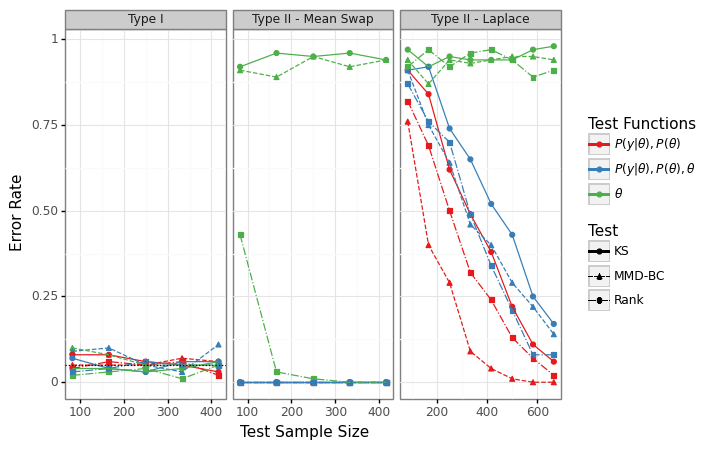
\includegraphics[width=\textwidth]{figures/gandy_scott_aux.png}
    \caption{Experiment 1 Type I/II error rates of BC tests with varying test functions, calculated over 100 trials with $\alpha=0.05$. In Algorithm \ref{alg:bc-sampler}, we set $M=5$. For the MMD-BC test, $\mathbf{\theta}$ test functions refer to $\{\theta_{1}, \theta_{2}\}$; for non-MMD tests, $\mathbf{\theta}$ test functions refer to $\{\theta_{1}, \theta_{2}, \theta_{1}^{2}, \theta_{1}\theta_{2}\}$. The MMD-BC test used the Gaussian kernel with bandwidth set using the median heuristic, with scale-normalized data. For the Rank test, we ordered test functions directly. For the MMD-BC and KS tests, `Test Sample Size' refers to the size of each sample seen by the tests. Though the Rank test is not a two-sample test, at a given `Test Sample Size', it runs roughly the same number of sampler iterations as the KS and MMD-BC tests.}
    \label{fig:ex1_aux}
\end{figure}

While the Type I error rates hover around the design parameter, without the auxiliary test functions, the Type II error rates for the MMD-BC and KS tests, shown in green, are stuck just below 1. Under the Mean Swap error, the marginal distributions of $\theta_{1}$ and $\theta_{2}$ are unchanged, so the two-sample tests relying solely on $\mathbf{\theta}$ test functions ($\{\theta_{1}, \theta_{2}\}$ for the MMD-BC test and $\{\theta_{1}, \theta_{2}, \theta_{1}^{2}, \theta_{1}\theta_{2}\}$ for the KS test) cannot detect this error. In the Laplace error, the posterior mean and variance are correct; because the $\mathbf{\theta}$-KS test only tests up to the second moments, it cannot detect this error either. Surprisingly, while the $\mathbf{\theta}$-MMD-BC test should be able to detect the Laplace error due the the characteristic nature of the Gaussian kernel, it seems to require a very high number of samples to do so.

These errors were chosen to be difficult to detect in $\mathbf{\theta}$-space. Consequently, the auxiliary test functions appear to capture the greatest discrepancies between samples. In the Laplace Error, the inclusion of the $\mathbf{\theta}$ test functions on top of the auxiliary test functions visibly increases the Type II error across all tests. This illustrates the trade-off inherent in enumerating test functions. Loosely speaking, each additional test function drastically improves detection rates for errors along that dimension, but reduces detection rates for discrepancies along orthogonal or sufficiently `distant' dimensions. In the Geweke and KS tests, this reduction in detection rates is driven by the multiple testing correction applied. For the MMD tests, this reduction occurs because the similarity between observations increases when irrelevant features are added.

The likelihood captures underlying structure in the model in a way that is otherwise difficult to characterize. We also attempted directly testing the equality of the joint distributions $P(\mathbf{Y}, \mathbf{\Theta})$ using the MMD tests using the Gaussian kernel with median heuristic (on scale-normalized samples). To be explicit, the test functions we used for this exercise (not shown) were $\mathbf{g}(\mathbf{\Theta}, \mathbf{Y}) = \begin{bmatrix}  \mathbf{Y}& \mathbf{\Theta} \end{bmatrix}^{\top}$, rather than \eqref{eq:testfn}. This approach was unable to detect the errors given the same computational budgets as in Figure \ref{fig:ex1_aux}. Computing separate Gaussian kernels on the data and parameters and using their sum or product as the test kernel was also ineffective.

% Appendix?
To the extent that the benchmark tests rely on a finite set of test functions, they are only able to examine discrepancies in a limited number of nonlinear features. In contrast, MMD-based tests are able to account for an infinite number of nonlinear features when using specific nonlinear kernels. Figure \ref{fig:ex1_kernel} illustrates the resulting benefits to power for the MMD-BC test. 
\begin{figure}
    \centering
    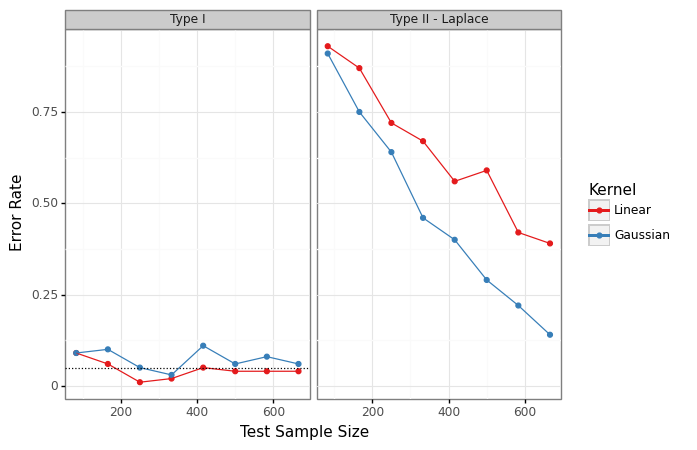
\includegraphics[width=\textwidth]{figures/gandy_scott_kernel.png}
    \caption{Experiment 1 MMD-BC Type I/II error rates using $\mathbf{\Theta}$ and the likelihood and prior auxiliary variables as test functions, calculated over 100 trials with $\alpha=0.05$. Algorithm \ref{alg:bc-sampler} set $M=5$. We used Gaussian kernels with median heuristic bandwidths on scale-normalized data.}
    \label{fig:ex1_kernel}
\end{figure}

The autocorrelation in the samples from Algorithm \ref{alg:sc-sampler} is extreme; though the Type II error rates are close to zero for the given hyperparameters, the SC tests require far more samples than the BC tests to push the Type I error rate below $\alpha=0.05$. Comparing efficiency across test types is not meaningful for the default parameters. However, we can reduce the autocorrelation by increasing $\sigma_{\epsilon}$ to obtain a fairer comparison. Turning this knob will allow us to analyze how the tests behave given samplers with varying mixing speeds. 
In Figure \ref{fig:ex1_auto}, we plot the Type I/II error rates for the correct sampler and the Laplace error sampler, holding both the total sampler iterations used by each test and the test sample sizes fixed. As we might expect, when the sample autocorrelation is very high, the SC tests always reject the null hypothesis. As $\sigma_{\epsilon}$ increases and the autocorrelation falls, the SC Type I error rates fall. In this plot, the SC Type I error rates generally exceed the BC test Type I rates; this is caused by high autocorrelation in the successive-conditional chains. However, note that for a given $\sigma_{\epsilon}$, we can reduce the MMD-SC and Geweke Type I error rates by thinning the chains.

As the autocorrelation decreases and mixing improves, the Type II error rates tend to decrease across the board. The exception to this trend is the initial spike experienced by the SC tests. As we move right from the leftmost extreme ($\sigma_{\epsilon} = 0.1$), the autocorrelation weakens enough that the SC tests sometimes fail to reject the null. Notably, the MMD-SC test exhibits better control of Type I error rates than the Geweke test here, despite the fact that both tests use Algorithm \ref{alg:sc-sampler}. On the other hand, the MMD-SC test is also less likely to correctly reject the null hypothesis. For $\sigma_{\epsilon} \geq 2.5$, the MMD-SC test has similar Type II error rates to the MMD-BC test. The KS test's Type II error rates lag behind the other tests in this setting.

\begin{figure}[H]
    \centering
    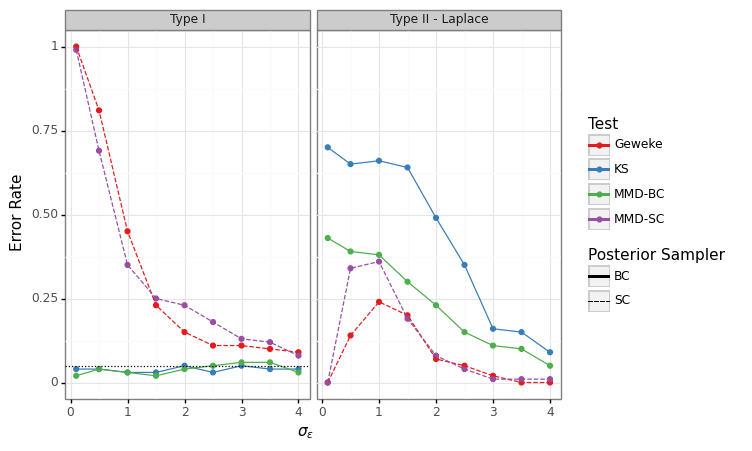
\includegraphics[width=\textwidth]{figures/gandy_scott_auto.png}
    \caption{Experiment 1 Type I/II error rates of BC and SC tests against $\sigma_{\epsilon}$, calculated over 100 trials with $\alpha=0.05$. As $\sigma_{\epsilon}$ increases, autocorrelation in the successive-conditional samples used in the Geweke and MMD-SC tests decreases. We allocated a budget of 1800 sampling iterations, keeping every 5th sample; each test received 300 samples from each sampler.}
    \label{fig:ex1_auto}
\end{figure}

\subsection{Reversible-jump Bayesian Lasso}
This example is based on \cite{chen_bayesian_2011}, but avoids using improper (hyper)priors in order to allow us to run Algorithm \ref{alg:mc-sampler}. We are interested in learning the parsimonious linear regression model
\begin{equation}
  \mathbf{y} = \mathbf{X}\mathbf{\beta} + \mathbf{\epsilon}, \quad \mathbf{\epsilon} \sim \mathcal{N}(\mathbf{0}, \sigma^{2} \mathbf{I})
\end{equation}
in a Bayesian setting. Rather than introducing an L1 penalty to the objective function with a corresponding regularization parameter as in frequentist Lasso, we instead promote sparsity by placing a truncated Poisson prior on the number $\ell$ of nonzero coefficients $\beta_{j}$, drawing $\ell$ coefficients from a Laplace distribution, and setting the remaining $p-\ell$ coefficients to zero. In addition, we place an inverse-gamma prior on $\sigma^{2}$. Let $\mathbf{\Theta} = \{\lambda, \sigma, \ell, \mathbf{\gamma}, \mathbf{\beta}\}$ denote the parameters, $\mathbf{X} \in \mathbb{R}^{n \times p}$ denote the (fixed) design matrix, and $\mathbf{y} \in \mathbb{R}^{n \times 1}$ denote the data. The prior is
\begin{equation}
  P(\mathbf{\Theta}|\tau, a, b ) = P(\ell|\lambda) P(\mathbf{\gamma}|\ell) P(\beta_{j} | \tau, \gamma) P(\sigma^{2} | a, b)
\end{equation}
\begin{equation}
  P(\ell|\lambda) = \frac{\exp{(-\lambda)} \lambda^{\ell}}{C\ell!}, \quad \ell \in \{1,\ldots, p\}
\end{equation}
\begin{equation}
  P(\mathbf{\gamma}|\ell) = {p\choose \ell}^{-1}
\end{equation}
\begin{equation}
  P(\beta_{j} | \tau, \gamma ) = \begin{cases} (2\tau)^{-1}\exp(-\frac{|\beta_{j}|}{\tau}) & j \in \mathbf{\gamma} \\ \delta(\beta_{j}) & \text{otherwise} \end{cases}
\end{equation}
\begin{equation}
    P(\sigma^{2} | a, b) = \frac{b^{a}}{\Gamma(a)} (\sigma^{2})^{-a-1} \exp{\left(-\frac{b}{\sigma^{2}}\right)}
\end{equation}
where $C$ is a normalization constant, $\delta$ is the Dirac delta function, and $\mathbf{\gamma}$ is a vector of the nonzero indices of $\mathbf{\beta}$.
The likelihood is given by
\begin{equation}
  P(\mathbf{y} | \sigma, \mathbf{\beta}, \mathbf{X} ) = (2\pi)^{-\frac{n}{2}} \sigma^{-n} \exp{\left(-\frac{\Vert\mathbf{y}-\mathbf{X}\mathbf{\beta}\Vert^{2}_{2}}{2\sigma^{2}}\right)}
\end{equation}
The joint probability is then
\begin{equation}
    \begin{aligned}
         P(\mathbf{y}, \mathbf{\Theta} | \mathbf{X} ) \propto &\sigma^{-n} \exp{\left(-\frac{\Vert\mathbf{y}-\mathbf{X}\mathbf{\beta}\Vert^{2}_{2}}{2\sigma^{2}}\right)} \times \\ 
         & \frac{\exp{(-\lambda)} \lambda^{\ell}}{\ell!} {p\choose \ell}^{-1} \prod_{j\in \mathbf{\gamma}} (2\tau)^{-1}\exp\left(-\frac{|\beta_{j}|}{\tau}\right) \prod_{j' \notin \mathbf{\gamma}} \delta(\beta_{j'}) \frac{b^{a}}{\Gamma(a)} (\sigma^{2})^{-a-1} \exp{\left(-\frac{b}{\sigma^{2}}\right)}
    \end{aligned}
    \label{eq:ex2_joint}
\end{equation}

Each iteration of the reversible-jump MCMC posterior sampler takes two steps in random order. The first is a Gibbs step, which is straightforward due to the conjugacy of the Inverse Gamma prior on $\sigma^{2}$.
\begin{equation}
    \sigma^{2} | \mathbf{y}, \mathbf{X}, \mathbf{\beta} \sim \mathcal{IG}\left(a + \frac{n}{2}, b + \frac{\sum_{i=1}^{n}(y_{i}-\mathbf{x}_{i}\mathbf{\beta})^{2} }{2}\right)
\end{equation}
where $\mathbf{x}_{i}$ denotes row $i$ of $\mathbf{X}$.

The second is a more involved reversible jump step. We start by proposing $\ell' \in \{\ell-1, \ell, \ell+1\}$ uniformly at random, disallowing $\ell<1$ and $\ell>p$. Thus, when $\ell \in \{1,p\}$, there are only two valid proposals, not three. Then, depending on the $\ell'$ proposed, we complete the proposal $\mathbf{\Theta}'$ via one of the following
\begin{itemize}
    \item Update: $\ell' = \ell$
    \begin{enumerate}
        \item Choose $j \in \{1, \ldots, \ell\}$ uniformly at random
        \item Propose $\mathbf{\gamma}' = \mathbf{\gamma}, \beta'_{j} = \beta_{j} + \mathcal{N}(0, \epsilon_{\text{update}}), \beta'_{i \neq j} = \beta_{i}$
        \item $P(\mathbf{\Theta}' \rightarrow \mathbf{\Theta}) = P(\mathbf{\Theta} \rightarrow \mathbf{\Theta}')=\mathcal{N}(\beta_{j}'; \beta_{j},\epsilon_{\text{update}})=\mathcal{N}(\beta_{j}; \beta_{j}',\epsilon_{\text{update}})$
    \end{enumerate}
\end{itemize}

\begin{itemize}
    \item Birth: $\ell' = \ell+1$
    \begin{enumerate}
        \item Choose $j \in \{\ell+1, \ldots, p\}$ uniformly at random
        \item Propose $\mathbf{\gamma}' = \mathbf{\gamma} \cup j$
        \item Propose $\beta'_{j} = \mathcal{N}(0, \epsilon_{\text{birth}}), \beta'_{i \neq j} = \beta_{i}$
        \item $P(\mathbf{\Theta}' \rightarrow \mathbf{\Theta}) = \begin{cases}\frac{1}{2}\frac{1}{\ell'} & \ell'=p \\ \frac{1}{3} \frac{1}{\ell'} & 1<\ell<p \end{cases} $
        \item $P(\mathbf{\Theta} \rightarrow \mathbf{\Theta}') = \begin{cases}\frac{1}{2}\frac{1}{p-\ell} \mathcal{N}(\beta_{j}'; 0,\epsilon_{\text{birth}}) & \ell=1 \\ \frac{1}{3} \frac{1}{p-\ell} \mathcal{N}(\beta_{j}'; 0,\epsilon_{\text{birth}}) & 1<\ell<p \end{cases} $
    \end{enumerate}
\end{itemize}

\begin{itemize}
    \item Death: $\ell' = \ell-1$
    \begin{enumerate}
        \item Choose $j \in \{1, \ldots, \ell\}$ uniformly at random
        \item Propose $\mathbf{\gamma}' = \mathbf{\gamma} \setminus j$ 
        \item Propose $\beta'_{j} = 0, \beta'_{i \neq j} = \beta_{i}$
        \item $P(\mathbf{\Theta}' \rightarrow \mathbf{\Theta}) = \begin{cases}\frac{1}{2}\frac{1}{p-\ell'} \mathcal{N}(\beta_{j}; 0,\epsilon_{\text{birth}}) & k'=1 \\ \frac{1}{3} \frac{1}{p-\ell'} \mathcal{N}(\beta_{j}; 0,\epsilon_{\text{birth}}) & 1<\ell'<p \end{cases} $
        \item $P(\mathbf{\Theta} \rightarrow \mathbf{\Theta}') = \begin{cases}\frac{1}{2}\frac{1}{\ell} & \ell=p \\ \frac{1}{3} \frac{1}{\ell} & 1<\ell<p \end{cases} $
    \end{enumerate}
\end{itemize}
where $\epsilon_{\text{update}}, \epsilon_{\text{birth}}$ are random walk sizes. We accept proposal $\mathbf{\Theta}'$ with probability $$A(\mathbf{\Theta}'|\mathbf{\Theta}) = \min{\left(\frac{P(\mathbf{y}, \mathbf{\Theta'} | \mathbf{X} )}{P(\mathbf{y}, \mathbf{\Theta} | \mathbf{X} )} \frac{P(\mathbf{\Theta}' \rightarrow \mathbf{\Theta})}{P(\mathbf{\Theta} \rightarrow \mathbf{\Theta}')}, 1\right)}$$

For this experiment, we fix the design matrix $\mathbf{X} \in \mathbb{R}^{1 \times 3}$, with $\lambda=1$ and hyperparameters $\tau=1, a=3, b=1$. The random walk sizes are set to $\epsilon_\text{update}= \epsilon_\text{birth}=1$.

\begin{table}[H]
    \centering
    \begin{tabular}{l|c|c|c}
          Error & Components & Incorrect & Correct \\
         \hline
         Transition & $A_{\text{birth}}(\mathbf{\Theta}'|\mathbf{\Theta})$, $A_{\text{death}}(\mathbf{\Theta}'|\mathbf{\Theta})$  &  $\min{\left(\frac{P(\mathbf{y}, \mathbf{\Theta'} | \mathbf{X} )}{P(\mathbf{y}, \mathbf{\Theta} | \mathbf{X} )}, 1\right)}$ & $\min{\left(\frac{P(\mathbf{y}, \mathbf{\Theta'} | \mathbf{X} )}{P(\mathbf{y}, \mathbf{\Theta} | \mathbf{X} )} \frac{P(\mathbf{\Theta}' \rightarrow \mathbf{\Theta})}{P(\mathbf{\Theta} \rightarrow \mathbf{\Theta}')}, 1\right)}$\\
         Poisson & $P(\mathbf{y}, \mathbf{\Theta'} | \mathbf{X} )$, $P(\mathbf{y}, \mathbf{\Theta} | \mathbf{X} )$ & $\ldots \frac{\exp{(-\lambda)} \lambda^{\ell}}{(\ell-1)!} \ldots$ & $\ldots \frac{\exp{(-\lambda)} \lambda^{\ell}}{\ell!} \ldots$ \\
    \end{tabular}
    \caption{Experiment 2 intentional errors in posterior sampler}
    \label{tab:ex2_errors}
\end{table}

We introduce several intentional errors into the the posterior sampler summarized in Table \ref{tab:ex2_errors}. The first error affects the Metropolis-Hastings acceptance probabilities used in the birth/death moves; it omits the jump probabilities $P(\mathbf{\Theta}' \rightarrow \mathbf{\Theta}), P(\mathbf{\Theta} \rightarrow \mathbf{\Theta}')$ from the calculation. The second error affects all of the Metropolis-Hastings acceptance probabilities. The $P(\ell|\lambda)$ factors of the joint probabilities have incorrect denominator $(\ell-1)!$ rather than $\ell!$. The results are shown in Figure \ref{fig:ex2_comparison}, with test functions shown in Table \ref{tab:ex2_testfn}.

\begin{table}[H]
    \centering
    \begin{tabular}{l|c|c|c|c}
         Test  & $\mathbf{\beta}, \sigma$ & $\{\mathbf{\beta}, \sigma\} \times \{\mathbf{\beta}, \sigma\}$ & $P(\mathbf{y}|\mathbf{\Theta}, \mathbf{X})$ & $P(\mathbf{\Theta})$ \\
         \hline
         MMD-SC & Y & & Y & Y \\
         MMD-BC & Y & & Y & Y \\
         Geweke & Y & Y & Y & Y \\
         KS & Y & Y & Y & Y \\
         Rank & Y & Y & Y & Y\\
    \end{tabular}
    \caption{Experiment 2 test functions}
    \label{tab:ex2_testfn}
\end{table}

The Type I error rates of the BC tests hover around the design parameter of $\alpha=0.05$, while the Geweke Type I error rates are elevated, at 19-25\%. The MMD-SC test has similar Type I error rates to the MMD-BC test. Note that these error rates, calculated using 100 trials, are relatively noisy.

For the two-sample tests, the Transition error is much easier to detect than the Poisson error, while the opposite is true for the Rank test.  Notably, while the Geweke test detects the Transition error quite easily, it essentially is unable to detect the Poisson error at the computation levels shown. In contrast, the other tests perform reasonably well, with Type II error rates that fall relatively quickly with sample size. 

Across both errors, we see that the MMD-SC test has lower Type II error rates than the MMD-BC test --- further evidence of the error magnification properties of Algorithm \ref{alg:sc-sampler}. The MMD-SC test most efficiently detects the Transition error, but lags behind the KS and Rank tests in detecting the Poisson error. The performance of the KS and Rank tests are quite consistent across both errors, with the KS test detecting the errors especially efficiently. This implies that the test functions accurately capture some of the discrepancies between samples.

\begin{figure}[H]
    \centering
    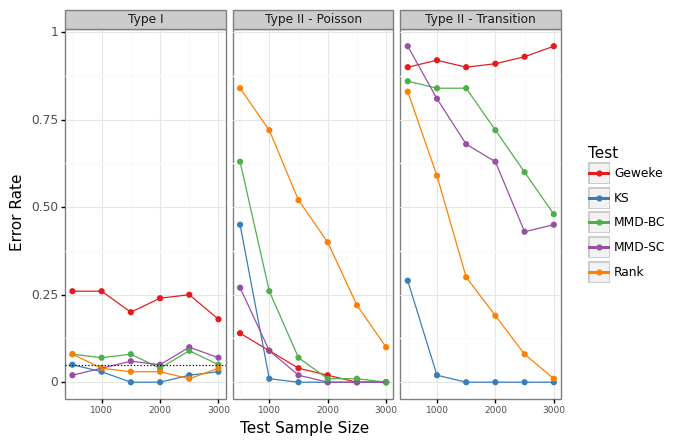
\includegraphics[width=\textwidth]{figures/bayes_lasso_comparison.png}
    \caption{Experiment 2 Type I/II error rates calculated over 100 trials with $\alpha=0.05$. Every $5^{\text{th}}$ sample from Algorithm \ref{alg:sc-sampler} was kept, and Algorithm \ref{alg:bc-sampler} set $M=5$. The MMD tests used Gaussian kernels with median heuristic bandwidths on scale-normalized data.}
    \label{fig:ex2_comparison}
\end{figure}

\subsection{Metropolis-Hastings for Learning DAG Structure}
In this experiment, we are interested in learning the structure of a directed acyclic graph (DAG) given observed data. See Figure \ref{fig:ex3_dag} for an example of a DAG.

\begin{figure}[H]
    \centering
    \begin{minipage}[b]{0.25\textwidth}
        \centering
        \usetikzlibrary{shapes.geometric}
        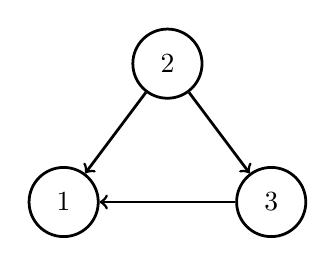
\begin{tikzpicture}
        [every node/.style={inner sep=0pt}]
        \node (1) [circle, minimum size=25.0pt, fill=white, line width=1pt, draw=black] at (112.5pt, -150.0pt) {\textcolor{black}{1}};
        \node (2) [circle, minimum size=25.0pt, fill=white, line width=1pt, draw=black] at (150.0pt, -100.0pt) {\textcolor{black}{2}};
        \node (3) [circle, minimum size=25.0pt, fill=white, line width=1pt, draw=black] at (187.5pt, -150.0pt) {\textcolor{black}{3}};
        \draw [line width=1, ->, color=black] (2) to  (1);
        \draw [line width=1, ->, color=black] (3) to  (1);
        \draw [line width=1, ->, color=black] (2) to  (3);
        \end{tikzpicture}
    \end{minipage}
     \begin{minipage}[b]{0.25\textwidth}
    \begin{align*}
        \begin{bmatrix}
            0 & 0 & 0 \\
            1 & 0 & 1 \\
            1 & 0 & 0 
        \end{bmatrix}
    \end{align*}
    \vspace{2ex}
    \end{minipage}
    \caption{Directed acyclic graph (DAG) with adjacency matrix representation. In the adjacency matrix, entry $(i,j)=1$ indicates the presence of a directed edge from node $i$ to node $j$; node $i$ is called a parent of $j$ and node node $j$ is called a child of node $i$. A node with no parents is called a root, and a node with no children is called a leaf.}
    \label{fig:ex3_dag}
\end{figure}

Let each observation on a root node $x_{r}$ be drawn from a normal distribution with standard deviation $\epsilon=1$, and let each child node be drawn from a normal distribution centered on the sum of its parents, also with standard deviation $\epsilon$. In other words, given graph structure $\mathcal{G}$ and data $\mathbf{X}$
\begin{equation}
    x_{r} \sim \mathcal{N}(0, \epsilon^2)
\end{equation}
\begin{equation}
    x_{j}|\mathbf{pa}(x_{j}) \sim \mathcal{N}(\sum_{z \in \mathbf{pa}(x_{j})} z, \epsilon^2)
\end{equation}
where $\mathbf{pa}(x)$ denotes the set of parent nodes of node $x$. Since the number of possible DAG structures is exponential in the number of nodes, for computational convenience, we consider all 3-node DAG structures.

Placing a uniform prior on $\mathcal{G}$, the posterior is proportional to the likelihood
\begin{equation}
    P(\mathcal{G}|\mathbf{X}) \propto P(\mathbf{X}|\mathcal{G}) = \prod_{i=1}^{n} \prod_{j=1}^{p} P(x_{ij}|\mathbf{pa}(x_{ij})) = \prod_{i=1}^{n} \prod_{j=1}^{p}
    \mathcal{N}(\sum_{z_{i} \in \mathbf{pa}(x_{ij})} z_{i}, \epsilon^2)
\end{equation}

The sampling algorithm we will consider is a modified version of the MCMC scheme from \cite{madigan_bayesian_1995} and is detailed in section 2 of \cite{grzegorczyk_improving_2008}. Given a graph structure $\mathcal{G}$, the proposal structure is sampled uniformly from the neighborhood of $\mathcal{G}$
\begin{equation}
P(\mathcal{G}' | \mathcal{G}) = \frac{1}{|\mathbf{Ne}(\mathcal{G})|}
\end{equation}
where the neighborhood $\mathbf{Ne}(\mathcal{G})$ is defined as the union of $\mathcal{G}$ and the set of all DAGs that can be reached by adding, deleting, or reversing an edge.

The Metropolis-Hastings acceptance probability is thus
\begin{equation}
A(\mathcal{G}'|\mathcal{G}) = \min{\left(1,\frac{P(\mathbf{X}|\mathcal{G}')|\mathbf{Ne}(\mathcal{G})|}{P(\mathbf{X}|\mathcal{G})|\mathbf{Ne}(\mathcal{G}')|}\right)}
\end{equation}

The sampler errors considered all affect the Metropolis-Hastings acceptance probability; specifically, they alter the calculation of $|\mathbf{Ne}(\mathcal{G})|$. In the first error, we count all \textit{graphs} that can be reached by modifying a single edge, regardless of whether the modification induces a cycle. In the second error, we double-count the DAGs that can be reached by reversing an edge. These errors are summarized in Table \ref{tab:ex3_errors}.

\begin{table}
    \centering
    \begin{tabular}{l|c|c|c}
          Error & Components & Incorrect & Correct \\
         \hline
         Cyclic Check & $|\mathbf{Ne}(\mathcal{G})|, |\mathbf{Ne}(\mathcal{G}')|$ & Count all graphs & Count all DAGs \\
         Rev Count & $|\mathbf{Ne}(\mathcal{G})|, |\mathbf{Ne}(\mathcal{G}')|$ & Count edge reversals twice & Count reversals once \\
    \end{tabular}
    \caption{Experiment 3 intentional errors in posterior sampler}
    \label{tab:ex3_errors}
\end{table}

We compare the MMD tests against the benchmark Geweke and Rank tests, with each test using the same set of manually engineered test functions (features) in a subset of $\mathbb{R}^{d}$. The MMD tests again use the Gaussian kernel with median heuristic bandwidth calculated on scale-normalized inputs. As a final benchmark, we include a $\chi^{2}$ test of the sample DAG frequencies. 

Most of the features are derived from the adjacency matrix representation of the sampled graph structure $\mathcal{G}$, shown in Figure \ref{fig:ex3_dag}. As an initial set of features, for all $i,j,i',j'$, we take
take each entry $(i,j)$, each $\mathrm{AND}((i,j),(i',j'))$, and each $\mathrm{XOR}((i,j),(i',j'))$. We then prune features that are exactly equal to other features or constant by construction. First, we remove features derived from duplicate edge pairs; for example, we keep only one of \{$\mathrm{AND}((i,j),(i',j'))$, $\mathrm{AND}((i',j'),(i,j))$\}. Next, diagonal entries $(i,i)=0$ are excluded (if they are nonzero, the graph is cyclic), along with all features derived from pairs with at least one diagonal entry. We also exclude $\mathrm{AND}((i,j),(j,i))=0$ and $\mathrm{XOR}((i,j),(i,j))=0$. Finally, we remove $\mathrm{AND}((i,j),(i,j)) = (i,j)$. As in the previous experiments, we also include the evaluation of the likelihood $P(\mathbf{Y}|\mathcal{G})$; the evaluation of the uniform prior $P(\mathcal{G})$ is omitted because it is constant.

\begin{figure}
    \centering
    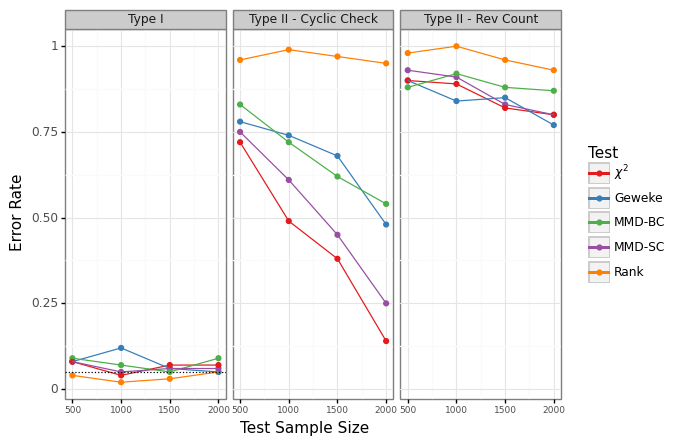
\includegraphics[width=\textwidth]{figures/graph_comparison.png}
    \caption{Experiment 3 Type I/II error rates calculated over 100 trials with $\alpha=0.05$. Every $5^{\text{th}}$ sample from Algorithm \ref{alg:sc-sampler} was kept, and Algorithm \ref{alg:bc-sampler} set $M=5$. The MMD tests used Gaussian kernels with median heuristic bandwidths on scale-normalized data. For the Rank test, we ordered test functions directly using a random tiebreak.}
    \label{fig:ex3_comparison}
\end{figure}

The results are shown in Figure \ref{fig:ex3_comparison}. Type I error rates are approximately what we would expect from the design parameter $\alpha=0.05$.

It is clear that the Rank test is inappropriate for this setting; it is unable to detect either error. For the other tests, the Cyclic Check error is much easier to detect than the Rev Count error. The $\chi^{2}$ test generally has the best detection rates, likely due to the fact that it operates directly on the space of DAGs rather than an incomplete representation in $\mathbb{R}^{d}$. Surprisingly, however, the MMD-SC test comes quite close to matching its ability to detect the Cyclic Check error. In the Rev Count error, the SC tests slightly lead the MMD-BC test in performance and match the $\chi^{2}$ test. Finally, we see once more that the MMD-SC test has lower Type II error rates than the MMD-BC test.

Another question we may ask is how much the use of a nonlinear kernel in the MMD tests buys us here, given that all but one of the features used are binary. Figure \ref{fig:ex3_kernel} suggests that the gains can be substantial. In the case of the Cyclic Check error, using the Gaussian kernel improves Type II by around 8\% across both tests. The effect on the Rev Count Type II error is unclear.

\begin{figure}
    \centering
    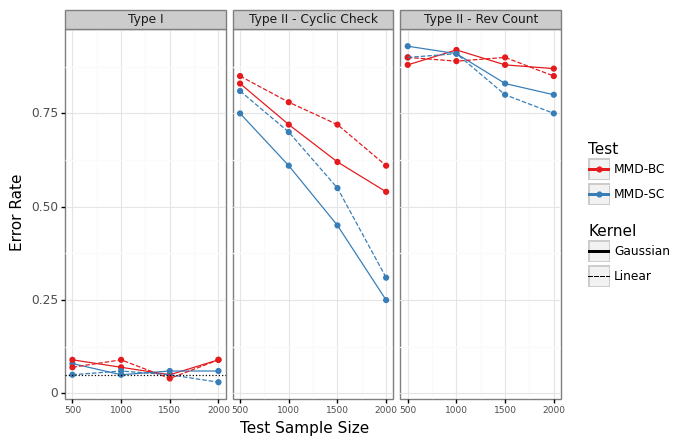
\includegraphics[width=\textwidth]{figures/graph_kernel.png}
    \caption{Experiment 3 Type I/II error rates calculated over 100 trials with $\alpha=0.05$ for MMD tests using linear/nonlinear kernels. Every $5^{\text{th}}$ sample from Algorithm \ref{alg:sc-sampler} was kept, and Algorithm \ref{alg:bc-sampler} set $M=5$.}
    \label{fig:ex3_kernel}
\end{figure}

It is important to emphasize that the tests as formulated are generally too expensive to conduct in richer DAG spaces; see the section \ref{section:discussion} for more details. It is possible, however, to adapt the MMD tests to these settings by using graph kernels; see \cite{kriege_survey_2020} for a survey. As a proof of concept we ran this experiment using random walk kernels \cite{gartner_graph_2003}, \cite{vishwanathan_fast_2006} in Figure \ref{fig:ex3_rw}. The kernels did not include any of our auxiliary test functions; combining data from different domains is another issue entirely. Using the random walk kernel, the MMD tests are able to detect the Cyclic Check error better than the $\chi^{2}$ test; however, the Rev Count Type II error degrades. In fact, random walk kernels cannot distinguish between isomorphic graphs. This illustrates a central issue with MMD; if a characteristic kernel is unavailable, MMD is not a metric on the space of probability distributions, and the test, however useful, will be inconsistent.

\begin{figure}[H]
    \centering
    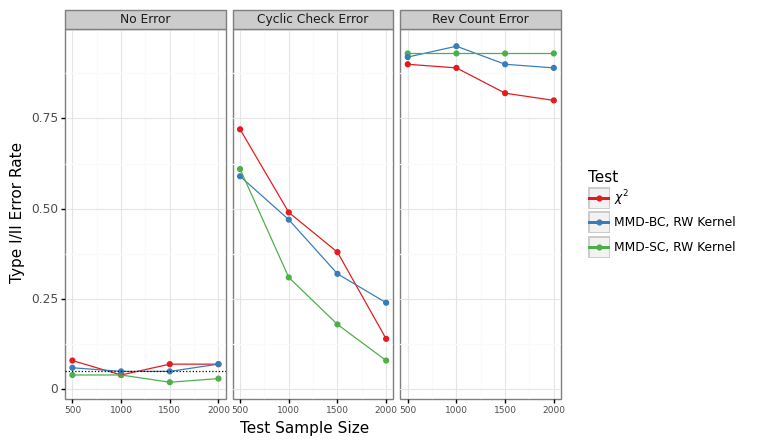
\includegraphics[width=\textwidth]{figures/graph_random_walk.png}
    \caption{Experiment 3 Type I/II error rates for MMD tests using the GraKeL \cite{siglidis_grakel_2020} random walk kernel implementation, with $\lambda=0.1$ and `geometric' summation. Calculated over 100 trials with $\alpha=0.05$. Every $5^{\text{th}}$ sample from Algorithm \ref{alg:sc-sampler} was kept, and Algorithm \ref{alg:bc-sampler} set $M=5$.}
    \label{fig:ex3_rw}
\end{figure}

\section{Discussion}
\label{section:discussion}
The MMD tests are preferable to existing tests from a theoretical perspective because they are able to directly test the null hypothesis that two distributions are the same, rather than approximating the null hypothesis via a family of sub-hypotheses. As we saw in experiment 1, Figure \ref{fig:ex1_aux}, for existing tests, the choice of test functions determines what errors can be detected. However, the MMD tests in a sense choose a collection of implicit test functions automatically based on their kernel. For example, a polynomial kernel of degree $d$ encodes all first to $d^{\text{th}}$ moments as `test functions' (features). In addition, the mean embeddings $\mathbf{\mu}_{P}$ and $\mathbf{\mu}_{Q}$ in an RKHS associated with a Gaussian kernel consist of the expectations of infinitely many features under distributions $P$ and $Q$, respectively. If any `test function' differs in expectation across $P$ and $Q$, it will contribute positively to the MMD. As discussed in \ref{section:testfn}, applying the Gaussian kernel to our particular choice of test functions \eqref{eq:testfn} results in a test that is not quite consistent, but scales better with the dimensionality of the data. The tests can easily be made consistent by ensuring that the test functions contain both the parameters and the data.

The infinite dimension of the mean embeddings is a double-edged sword in the sense that testing all features at once reduces the interpretability of the test. If the null hypothesis is rejected, we do not know which features drove the rejection and we are left none the wiser about where the error might be. In contrast, testing a family of user-specified test functions non-MMD tests, may allow the user to pinpoint the block of parameters in which the error lies. For example, in experiment 2, the rejected test functions all concern $\mathbf{\beta}$ rather than $\sigma$, telling us correctly that the errors are not in the $\sigma$ Gibbs step.

Naturally, the choice of kernel $k$ has a significant impact on the performance of the MMD tests. In experiments 1 and 3, we saw that using a nonlinear kernel generally improved Type II error rates over a linear kernel for both tests; the exception was in the Rev Count error in experiment 3, where the effect was ambiguous. It is reasonable that Type II error rates would benefit from the use of the Gaussian kernel in particular; the linear kernel only takes into account features we provide to it, while the Gaussian kernel takes an infinite number of features into account. Further, unlike the linear kernel, the Gaussian kernel is universal and thus characteristic on $\mathbb{R}^{d}$, and any difference between two probability distributions will manifest in the associated MMD test.

We exploited the universality of the Gaussian kernel in experiment 3 by mapping graph structures to sets of binary features (test functions) in $\mathbb{R}^{d}$. By \cite{christmann_universal_2010}, Theorem 2.2, as long as this mapping is one-to-one, the Gaussian kernel is universal on the embedding. Many graph kernels take a similar approach, inducing an explicit feature vector and then applying a linear kernel. The fact that applying the Gaussian kernel improves test power in experiment 3 compared to the linear kernel, as shown in Figure \ref{fig:ex3_kernel}, implies that our features do not fully capture the underlying graph structures. This evokes similar results in the literature showing that using nonlinear decision boundaries on explicit feature vectors induced by graph kernels can improve performance \cite{kriege_survey_2020}. 

Further, the feature vectors used in experiment 3, however lacking, are still challenging to deal with from both computational and statistical perspectives. In experiment 3 specifically, the number of features is exponential in the number of nodes. In our case, with just over 30 features characterizing 3-node graphs, this is manageable. However, for even moderately-sized structures, just computing the feature vector for one sample becomes difficult. For example, 30-node graphs yield over 750,000 features. Even if it were feasible to compute the feature vectors for each sample, multiple testing corrections would significantly reduce test power. The $\chi^{2}$ test also does not scale well; the number of possible DAGs is also exponential in the number of nodes. In contrast, the MMD tests easily scale in this setting given the right choice of graph kernel. The trade-off is instead that it is difficult to prove that kernels are characteristic on graphs. As we saw in Figure \ref{fig:ex3_rw}, the random walk kernel in particular is unable to detect the Rev Count error, while the Gaussian kernel can.

In $\mathbb{R}^{d}$, the MMD tests perform competitively compared to existing tests of the same class. However, they are much more expensive to conduct, with computational costs quadratic in the number of observations rather than linear or log-linear. In particular, the MMD-SC test exhibits better control of Type I error rates than the Geweke test, which also uses Algorithm \ref{alg:sc-sampler}, in experiments 1 and 2. However, as we can see in experiment 2, it is able to detect errors that the Geweke test cannot. On the other hand, in our experiments, the MMD-BC test does not have a clear performance advantage over other tests using Algorithm \ref{alg:bc-sampler}. As we might expect, the independent sample tests' Type I error rates are quite similar. However, the Type II error rates differ quite dramatically by experiment and by error. The MMD test outperforms the KS test in experiment 1, but not in experiment 2; it is outperformed by the Rank test in experiment 1 and in the Poisson error of experiment 2, but not in the transition error of experiment 2 and experiment 3. 

The inconsistency in the MMD-BC test's Type II error rates relative to other tests based on Algorithm \ref{alg:bc-sampler} may be driven by differences in the effects of increasing dimensionality. This is illustrated in the rightmost facet of Figure \ref{fig:ex1_aux}. Under the alternative hypothesis, assume a subset of test functions sufficiently captures some of the discrepancies between samples such that the corresponding null hypotheses are rejected. In the Laplace error of experiment 1, this subset of test functions is $\{P(\mathbf{y}|\mathbf{\theta}), P(\mathbf{\theta})\}$. Using only this subset of test functions for hypothesis testing results in the greatest power for each test; for example, see the red lines in Figure \ref{fig:ex1_aux}. However, in practice, we do not know where the error will manifest ahead of time. The non-MMD tests lose power from testing features outside of the subset due to multiple testing corrections. As the number of features increases, MMD tests also lose power \cite{reddi_decreasing_2014} --- the curse of dimensionality. In the Laplace error in particular, comparing the red and blue lines in Figure \ref{fig:ex1_aux}, we see that the MMD-BC test loses power more quickly from increasing dimensionality than the KS and Rank tests. This suggests that if the number of rejecting test functions is small relative to the total, then the MMD tests will perform poorly relative to existing tests. 

In addition to the implicit features encoded in the chosen kernel, as we saw in experiment 1, including hand-picked features in the MMD test can significantly improve detection rates. The features we chose were the likelihood and prior evaluated on the sample. In particular, these capture the relationship between the data and parameters much better than including the data as test functions directly in experiment 1. The likelihood and prior are especially good choices for test functions because their dimensionality is fixed, and do not significantly reduce the power of the tests if they prove irrelevant, even when the data are very high-dimensional.

If we are given a choice between the MMD-SC and MMD-BC tests, which one should we pick? The answer depends on how much we value accuracy versus speed. The MMD-SC test is preferable for accuracy. In experiments 2 and 3, we saw that it was significantly better at detecting errors than the MMD-BC test, while keeping the Type I error rates similar. On the other hand, this improved performance comes at a potentially steep cost. The results of experiment 1, Figure \ref{fig:ex1_auto}, showed us that high autocorrelation in the samples (slow mixing in the posterior sampler) drawn by Algorithm \ref{alg:sc-sampler} hamstrings the MMD-SC test. In order to control the Type I error rate under this regime, we must draw many more, heavily thinned samples. relative to the MMD-BC test. 

In terms of speed, the MMD-BC test is the clear winner. The MMD-SC and MMD-BC tests are quite similar in raw operation count. Assume we have an equal number of samples $N$ from Algorithms \ref{alg:mc-sampler}, \ref{alg:sc-sampler}, and \ref{alg:bc-sampler}. Let $K$ denote the cost of computing the kernel on one pair of observations, let $B$ denote the number of bootstrapped statistics generated. In the experiments we conducted, we kept the number of samples drawn constant. Computing the biased statistic \eqref{eq:mmd_biased} used in the MMD-SC test is $O(3KN^{2})$, while computing the unbiased statistic \eqref{eq:mmd_unbiased} is $O(3KN^{2}-2KN)$. Computing the wild and permutation bootstrapped statistics both cost $O(3N^{2})$. The main computational difference between the MMD-SC and MMD-BC tests is in their ability to be parallelized. The samples from Algorithm \ref{alg:sc-sampler} must be drawn in sequence if they are to amplify errors; we cannot take advantage of more than two threads. In contrast, since each sample from Algorithm \ref{alg:bc-sampler} is independent, we can use up to $N$ threads.

\section{Conclusion}

In this study, we have introduced two new MMD-based tests for checking the correctness of MCMC algorithms. These tests offer several advantages over existing tests. First, the tests are correctly specified, directly testing the two-sample null hypothesis. As a result, the tests generally exhibit better sample efficiency than the commonly-used Geweke test and perform on par with newer tests, but in some cases lag behind the latter. Second, the tests are generalizable to more abstract domains such as graphs, while all current alternatives are not (in nontrivial cases). On the other hand, the MMD tests are generally more computationally intensive than competitors.

We have demonstrated the efficacy of the MMD tests in three significantly different settings --- a toy Gibbs sampler, a reversible-jump Bayesian Lasso, and structure-MCMC via Metropolis-Hastings. In particular, we showed the advantages of encoding pre-existing knowledge specific to MCMC into the kernel, using test functions corresponding to the likelihood and prior. We also showed that these advantages could be further amplified by using nonlinear instead of linear kernels. Finally, we showed that the MMD tests have different properties. The user should keep in mind that the MMD test based on the successive-conditional simulator exhibits lower Type II error rates than the backwards-conditional MMD test, at the cost of potentially elevated Type I error rates when samples are highly autocorrelated.

\subsection{Future Research}
We see four directions for future research. The first is the construction of better comparisons across tests through tighter control of computational costs. Commonly used approximations based on CPU wall time have several disadvantages. In this study, we only controlled for the number of samples drawn to conduct each test; however, this inherently advantages the MMD tests, which are more expensive to conduct given the same sample size. More accurate comparisons between tests would allow researchers to better determine which to choose.

The second direction is finer optimization of test parameters to maximize test power. Here, we have used the median heuristic for the Gaussian kernel due to its sample efficiency. However, we may be able to do better using other methods, including those which learn the kernel parameters on a training set perform the test on a held-out test set. For instance, we might maximize the t-statistic from \cite{sutherland_generative_2019}.

The third direction is further extension of the MCMC MMD tests to domains other than $\mathbb{R}^{d}$. One challenge in this area is figuring out how to combine test functions from different domains. In particular, the likelihood and prior test functions are in $\mathbb{R}^{d}$, while the parameters are not. While we could just ignore the likelihood and prior test functions entirely, we ideally would like to exploit the information they contain. A potential solution would be to simply compute separate kernels for the auxiliary test functions and the parameters, then use their product as the test kernel.

The final direction is generalizing our MCMC test frameworks to other methodologies. A straightforward extension is assessing approximate MCMC algorithms; for a review, see \cite{bardenet_markov_2015} section 6. Approximate MCMC algorithms, when the underlying dataset is large, achieve substantial speed gains over their exact counterparts by estimating acceptance ratio likelihood terms, reducing variance at the cost of introducing asymptotic bias. By simply swapping out the posterior sampler in Algorithms \ref{alg:mc-sampler}, \ref{alg:sc-sampler}, and \ref{alg:bc-sampler} for an approximate version, our tests can be used directly to evaluate the validity of the schemes. We may also be able to apply the two-sample approach in approximate Bayesian computation (ABC) methods, which simulate the posterior via likelihood-free rejection sampling; see \cite{grazian_review_2020} for a review.

\bibliographystyle{apalike}
\bibliography{references}

\end{document}